\documentclass{article}
\usepackage[hidelinks]{hyperref}
\usepackage{csquotes}
\usepackage[vmargin=25mm, hmargin=20mm]{geometry}
\usepackage{xcolor}
\usepackage{graphicx}
\usepackage{float}
\usepackage{pgfplots}
\usepgfplotslibrary{colorbrewer}
\pgfplotsset{compat = 1.18} 
\usetikzlibrary{pgfplots.statistics, pgfplots.colorbrewer} 
\usepackage{pgfplotstable}
\usepackage{listings}
\lstset{
    backgroundcolor=\color[RGB]{240, 240, 240},   
    basicstyle=\ttfamily\footnotesize,
    breakatwhitespace=false,
    breaklines=true,
    keepspaces=true,
    numbers=left,
    numbersep=5pt,
    showspaces=false,
    showstringspaces=false,
    showtabs=false,
    tabsize=4,
    postbreak=\mbox{\textcolor{red}{$\hookrightarrow$}\space},
    aboveskip=10pt
}
\usepackage[
    backend=biber,
    sorting=none,
    style=ieee,
    urldate=long,
    maxcitenames=2,
    mincitenames=1
]{biblatex}
\addbibresource{sources.bib}
\renewcommand*{\bibfont}{\footnotesize}
\usepackage{multicol}
\setlength{\columnsep}{13mm}
\usepackage{hypcap}
\usepackage{caption}
\captionsetup{
    justification=centerlast,
    font=small,
    labelfont=sc,
    margin=5pt,
    belowskip=15pt
}
\DeclareCaptionType{listing}[Listing][List of Listings]
\renewcommand{\arraystretch}{1.5} % Increase table padding


\title{%
\vspace{50px}%
    \Huge Differential Fuzzing on coreutils Using LibAFL\break%
    —\break%
    Report%
    \vspace{250px}%
}

\author{%
  Valentin Huber\vspace{5px}\\%
  \small \href{https://www.zhaw.ch/en/engineering/institutes-centres/init/}{Institute of Applied Information Technology}\\%
  \small \href{https://www.zhaw.ch/en}{Zürich University of Applied Sciences ZHAW}\\%
  \small \href{mailto://contact@valentinhuber.me}{contact@valentinhuber.me}%
  \vspace{10px}
}
\date{\today\vspace{5px}}

\DeclareFieldFormat*{citetitle}{\textit{#1}}
\hfuzz=50px
\hbadness=10000
\newcommand{\code}[2][]{\lstinline[language=#1, breaklines=false, basicstyle=\ttfamily\normalsize]{#2}}
\let\savedCite=\cite
\renewcommand{\cite}{\unskip~\savedCite}

\begin{document}
\pagenumbering{gobble}
\maketitle

\clearpage\newpage
\begin{center}
    \begin{minipage}{0.8\textwidth}

        \vspace{70px}

        \begin{abstract}
            While fuzzing has become an important technique to ensure software reliability and security, the oracles used by most fuzzers to detect software errors are limited to very simple heuristics such as software crashes. To identify more nuanced logic errors, researchers have introduced differential fuzzing, which incorporates checks on the discrepancies between the outputs of two implementations of the same logic under the same input into the fuzzer's oracle. %
            %
            The coreutils suite of programs represents a fundamental component of the UNIX operating system, providing a foundation for users to interact with their operating system through the command line interface. While the version of coreutils developed by the GNU project is the most prevalent, alternative implementations, such as those developed by the uutils project, are also available. %
            %
            The LibAFL is a fuzzing framework was developed with the intention of improving compatibility between improvements to different parts of fuzzers and provides basic support for differential fuzzing.

            This work builds upon the foundations laid by LibAFL to create a differential fuzzer that can be run on different implementations of coreutils. It introduces a novel coverage instrumentation on GNU's and uutils' version of coreutils, a coverage gathering and transfer method idiomatic to LibAFL's coverage guidance system, and improvements to the differential fuzzing subsystem. %
            %
            Due to current limitations in LibAFL's input mutators, evaluation was conducted solely on \code{base64}, where the fuzzer achieved full code coverage and any artificially introduced logic errors were promptly and reliably identified. %
            %
            This system implements a trade-off between completeness and performance, whereby subtle logic errors can be identified by focusing on testing programs' business logic and ignoring functionality that changes the testing environment or is related to \code{stdio} handling.
        \end{abstract}
    \end{minipage}

    \vspace{70px}

    \begin{minipage}{0.7\textwidth}
        \textbf{Keywords}: Software Testing, Fuzzing, Differential Fuzzing, coreutils, LibAFL.
    \end{minipage}
\end{center}

\clearpage\newpage

\pagenumbering{arabic}
\begin{multicols}{2}
    \tableofcontents

    \section{Introduction}

    Fuzz testing has become an important tool for finding software defects. By repeatedly running a program under test with varying input data and detecting illegal states such as crashes, it is an automated alternative to manual security and reliability testing. Introduced in \citeyear{UNIX} in the seminal work by \citeauthor{UNIX}\cite{UNIX}, it is now widely used in industry. Companies such as Google, Microsoft, Cisco and Adobe, and government agencies such as the US Department of Defense, have developed proprietary fuzzers or contributed to open source fuzzers. Fuzz testing has proven to be an effective tool for both security and reliability testing. It has been credited with finding 20,000 vulnerabilities in Google's Chrome browser alone.\cite{Demystifying}

    \subsection{Differential Fuzzing}
    \label{IntroductionDifferentialFuzzing}

    While fuzzing has been extensively researched, one area that has not received much attention is the oracle that defines what constitutes an illegal state of the program under test. While simple oracles such as program crashes and timeouts are easy to detect, further research has not gone beyond very general logic, such as memory corruption bugs.\cite{SurveyRoadmap}

    One such oracle is the one used in so-called differential fuzzing. It relies on two independent implementations of the same underlying program logic and works by comparing their output under the same input. Compared to other common and more general oracles, this allows for the detection of subtle logic errors that do not invalidate basic guardrails such as memory access rules.

    \subsection{coreutils}

    This paper examines coreutils as an example of a target for differential fuzzing. coreutils is a suite of programs that allow users to interact with their system from the command line. Popularised by the version developed by the GNU project and available on almost all current Linux systems, utilities such as \code{ls}, \code{cat}, \code{base64}, \code{grep}, \code{env} or \code{whoami} are essential tools for many users' daily work. Section~\ref{Coreutils} provides a more detailed introduction to coreutils, including information about its history, interface and technical build-up.

    \subsection{LibAFL}
    \label{LibAFLHistory}

    American Fuzzy Lop (AFL)\cite{AFL} was an early comprehensive open source fuzzing tool used in countless projects and academic papers. By combining compile-time coverage instrumentation and genetic mutation of inputs that triggered new code paths, it proved to be a very effective at finding software bugs and vulnerabilities\cite{AFLBugs}. After it ceased to be updated in November 2017, the fork AFL++\cite{AFLPlusPlus} has become the de facto replacement.

    However, while enhancements to AFL++ have been introduced in many academic and commercial projects, due to the architecture of AFL++, these enhancements have usually not been merged back into AFL++. The result is a list of incompatible forks, each with a proven improvement that makes the fuzzer more effective at its job.\cite{LibAFL} Because of this, the maintainers of AFL++ have started a new project: LibAFL. It aims to provide a toolkit for building fuzzers that is flexible enough to allow the combination of all these improvements. Refer to Section~\ref{LibAFLBackground} for more details on LibAFL. This work uses LibAFL to build a fuzzer aimed at finding software bugs in coreutils.

    \subsection{Research Questions}
    \label{ResearchQuestions}

    The remainder of this work aims to answer the following questions:

    \begin{enumerate}
        \item Which parts of coreutils can be fuzzed? What are the performance trade-offs required for each part?
        \item How can the necessary instrumentation be introduced into coreutils? What are the engineering and performance implications of each option?
        \item Is it feasible to use LibAFL to build a system with all the logic defined in the answers to the above questions?
        \item If so, how effective is the resulting fuzzer at finding bugs in coreutils? What kind of bugs can it find?
        \item Can the system be extended to perform differential fuzzing between the different implementations? What changes need to be made?
        \item If so, how effective is this second fuzzer at finding bugs in coreutils? What kind of bugs can it find?
    \end{enumerate}

    Refer to Section~\ref{ResearchQuestionsDiscussion} for a summary of the answers given in this paper.

    \section{Background}

    To understand the requirements and architecture of the fuzzer, some background information on coreutils and the architecture of LibAFL is necessary. This section gives an overview of these topics.

    \subsection{coreutils}
    \label{Coreutils}

    On \citedate{FileUtilsAnnouncement}, {\DeclareNameAlias{labelname}{given-family}\citeauthor{FileUtilsAnnouncement}} announced fileutils, a suite of utilities for reading and modifying files\cite{FileUtilsAnnouncement}. A year later, he released textutils (for parsing and manipulating text)\cite{TextUtilsAnnouncement} and shellutils (for writing powerful shell scripts)\cite{ShellUtilsAnnouncement}. These three collections were merged into one on \citedate{CoreUtilsAnnouncement}, called GNU coreutils.\cite{CoreUtilsAnnouncement} \code{ls}, \code{cat}, \code{base64}, \code{grep}, \code{env}, or \code{whoami}: GNU's coreutils are the foundation of how users interact with most Linux distributions at the command line.\cite{GNULinux} Because they are so widely used and central to how users interact with their computers, software quality and the absence of software bugs are particularly important for coreutils.

    Version 9.5 of the GNU coreutils was released on \citedate{GNUCoreUtils9.5} and thus marks the current version as of this report. 106 programs are built by default.\cite{GNUCoreUtils9.5}

    \subsubsection{Interface}
    \label{CoreutilsInterface}

    Users interact with coreutils primarily through the command line or in shell scripts. They take different kinds of input, i.e. behave differently based on changes to:

    \begin{itemize}
        \item Data passed to \code{stdin}, e.g. through UNIX pipes
        \item Command line arguments:
              \begin{itemize}
                  \item Unnamed arguments, either required (such as \code{cp <source> <destination>}) or optional (such as \code{ls [directory]})
                  \item Flags without any associated data, such as \code{--help}
                  \item Flags with associated data, either required (such as \code{dd} \code{if=<input file>} \code{of=<output file>}) or optional {such as \code{-name <pattern>} in \code{find}}
              \end{itemize}
        \item Environment variables, such as \code{LANG}
        \item File system content, such as for \code{ls}
    \end{itemize}

    The output, or effects of invocations fall into the following categories:
    \begin{itemize}
        \item Data written to \code{stdout}
        \item Data written to \code{stderr}
        \item The exit status of the process
        \item The signal terminating the process
        \item Changes to the file system
    \end{itemize}

    \subsubsection{Alternative Implementations}

    Since the release of GNU coreutils, numerous alternative implementations have been released. Among these, BusyBox stands out as a notable example. Its objective is to provide a substantial subset of the GNU coreutils, with a particular focus on resource restrictions. Consequently, it is primarily employed in embedded systems\cite{BusyBox} or in tiny distributions such as Alpine Linux\cite{Alpine}.

    In the general trend of rewriting software in memory-safe languages, the uutils project\cite{Uutils} maintains a drop-in replacement implementation of the GNU coreutils written in Rust. This implementation contains all programs, but is still missing certain options. All differences with GNU's coreutils are treated as bugs. Furthermore, the project aims to not only work on Linux, but also on MacOS and Windows.

    \subsubsection{Build System}
    \label{CoreutilsBuildSystem}

    The GNU coreutils employ a complex, multi-step build system, including Autoconf\cite{Autoconf} and Automake\cite{Automake}. Any changes to either the code or the build system configuration require a deep understanding of the entire ecosystem to ensure that no unintended changes to the resulting binaries are introduced. The version of coreutils provided by uutils relies on cargo as its build system, which makes the outcomes of changes to the code much more predictable.

    \subsection{LibAFL}
    \label{LibAFLBackground}
    As previously outlined in Section~\ref{LibAFLHistory}, LibAFL is an extendible framework for the construction of custom fuzzers. This section will provide a brief introduction to the fundamental concepts and components of LibAFL that are essential for an understanding of this project. For a more comprehensive examination, the authors direct the reader to the original LibAFL paper\cite{LibAFL}.

    \subsubsection{Generic Concepts}
    The core insight of the authors of LibAFL is that the majority of fuzzers contain highly similar components, with advancements in new works typically occurring in only a few of the fundamental fuzzer parts.

\end{multicols}
\vspace{1em}
\begin{figure}[b]
    \centering
    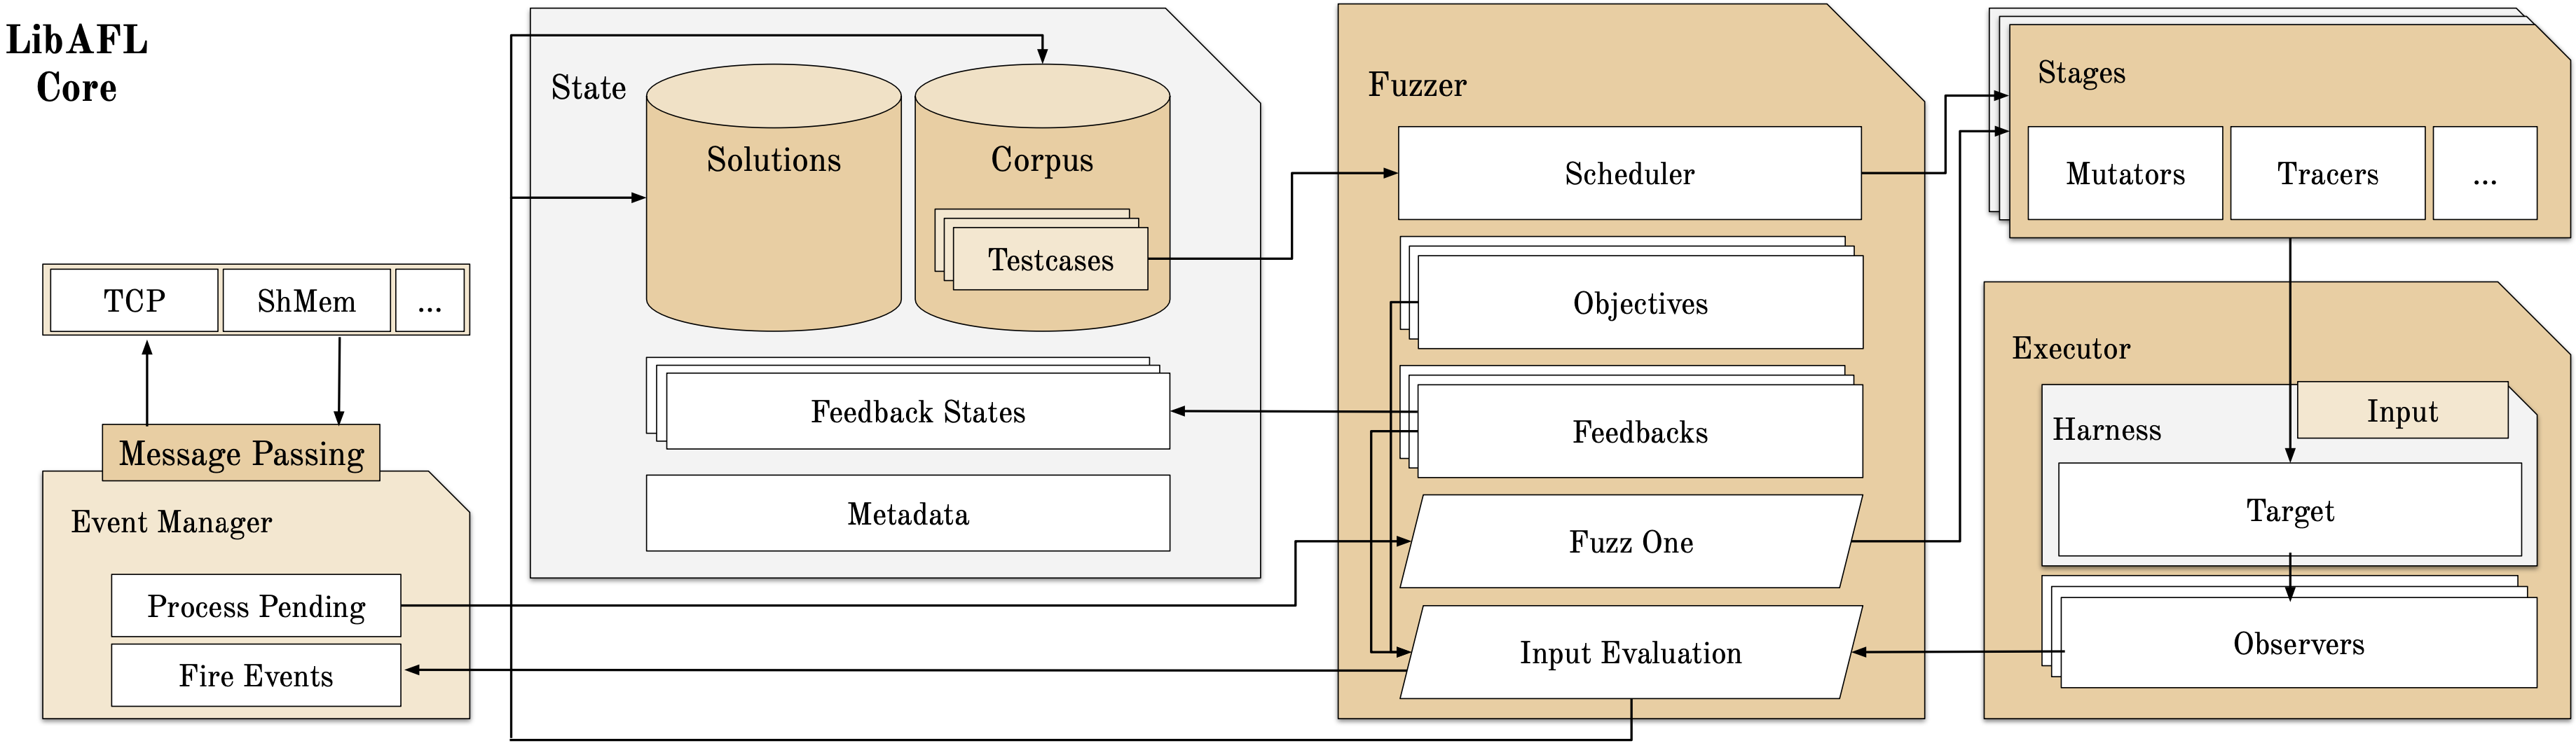
\includegraphics[width=\textwidth]{assets/LibAFLArchitecture.png}
    \caption{LibAFL's Architecture\cite{LibAFL}}
    \label{fig:LibAFLArchitecture}
\end{figure}
\begin{multicols}{2}

    This logic is typically introduced into a fork of an existing fuzzer (such as AFL++), which is then abandoned without the advancements being collected in a way that allows them to be reusable and combinable in later projects. An alternative approach is to create a new system from scratch, which introduces a significant amount of duplicate work and code that may not be as optimised as possible. This is because fuzzer parts such as thread synchronisation are not typically the focus of new works.

    The authors of LibAFL conducted a comprehensive examination of recent innovations in fuzzing and identified a set of distinct parts present in numerous fuzzers. They then designed the architecture of LibAFL in such a way that authors can modify only the parts they are interested in while relying on a well-optimised default implementation for everything else. Figure~\ref{fig:LibAFLArchitecture} illustrates the identified fuzzer parts and their interaction, as implemented in LibAFL. The authors of LibAFL re-implemented the logic introduced in 20 high-impact works to demonstrate that the system is flexible enough to handle logic created independently of their system. Finally, they showed that it is now trivial to combine advancements made in different works (i.e. combining the input scheduler of one work with new feedback types introduced in another).

    \subsubsection{Usage of Traits}
    \label{LibAFLTraits}

    From a technical standpoint, the authors' objective was achieved through the utilisation of Rust's trait system in conjunction with generic types. This section will present a selection of these core traits, accompanied by a brief explanation. For a comprehensive list and more comprehensive documentation, the author refers to the paper that introduced LibAFL\cite{LibAFL} and the official LibAFL book\cite{LibAFLBook}.

    \paragraph{Executor}

    The \code{Executor} is invoked with a certain \code{Input} and executes the program under test. It ensures that the passed \code{Observer}s can gather whatever information they need to and provide additional information about the execution run. Examples of \code{Executor}s include \code{InProcessExecutor}, which calls the provided function directly, and \code{InProcessForkExecutor}, which calls \code{fork} before calling the function and trades off additional performance overhead for improved stability. Finally, while being libraries external to the LibAFL core, \code{FridaInProcessExecutor} and \code{QemuExecutor} utilise the dynamic instrumentation framework Frida and the emulator QEMU, respectively, to support complex fuzzing approaches.

    \paragraph{Observer}

    \code{Observer}s are passed to an \code{Executor} and gather information before, during, or after the execution. This information can take any arbitrary shape. Typical \code{Observer} implementations used in fuzzers include \code{StdMapObserver}, which is often used to keep track of coverage data by recording execution paths, or \code{CmpObserver}, which is used to trace comparisons during an execution run.

    \paragraph{Feedback}

    There are two principal applications for \code{Feedback}s in LibAFL: objectives and feedbacks steering the search. In both cases, a \code{Feedback} reduces a combination of information provided by the \code{Executor} and \code{Observer}s to a Boolean value: Is this test case deemed to be interesting? When used as an objective, this marks the test case in question as a solution. When employed as a steering feedback, it will append the current test case to the corpus from which (after mutating it) the next input is drawn. Typical examples include \code{CrashFeedback}, \code{TimeoutFeedback} (both usually used in the objective mode) and \code{MaxMapFeedback}, which may be utilized to ascertain whether new portions of the memory map utilized to monitor the executed segments of the binary are accessed, thereby representing the coverage-guided aspect of the fuzzer.

    \paragraph{Input}

    \code{Input}s represent data that is mutated and subsequently passed to the \code{Executor}. It typically comprises a simple variable-length byte array, although it may also be a more complex \code{struct}. Depending on the specific use case, the former may be sufficient, or the latter may be required to provide additional flexibility.

    \paragraph{Mutator}

    Finally, \code{Mutator}s take an \code{Input} and modify it in some way. In the case of simple byte array \code{Input}s, this may involve inverting a bit or inserting an additional byte. For more complex \code{Input}s, custom \code{Mutator}s may need to be written. All \code{Mutator}s included in a certain fuzzer are passed to a scheduler, which mutates an \code{Input} once or multiple times with the received \code{Mutator}s. This is another example of the flexibility of LibAFL: While one may need to write custom \code{Mutator}s for a custom \code{Input} type, all scheduling algorithms available in LibAFL can be used regardless, without any additional changes.

    \section{Implementation}
    \label{Implementation}

    This section introduces the concepts and technical details necessary to reproduce the findings of this work by incrementally adding capabilities to a fuzzer. The example fuzzer will target \code{base64}, a comparatively small program from the coreutils. It encodes and decodes binary data to a format consisting only of characters unproblematic in most contexts. It takes its input from either a file or \code{stdin} and provides the following options:
    \begin{itemize}
        \item \code{--decode} switches \code{base64}'s mode from encode to decode
        \item \code{--ignore-garbage} ignores non-alphabet characters when decoding
        \item \code{--wrap <cols>} inserts linebreak after \code{<cols>} characters when encoding
        \item \code{--help} prints information about \code{base64} and exits
        \item \code{--version} prints version information and exits
    \end{itemize}

    \subsection{Basic Unguided Fuzzer}

    The initial step is to construct a fuzzer devoid of any features. It merely takes a byte array, randomly mutates it, feeds it to the program under test and checks for crashes. It does not contain any execution steering nor can it trigger the different options. One can select the default implementations for each part outlined in Section~\ref{LibAFLBackground}, which reduces the necessary code for the fuzzer to well under 100 lines. However, it is unlikely that this fuzzer will identify any software defects, as it employs a strategy similar to that proposed in the seminal work by \citeauthor{UNIX} in \citeyear{UNIX}\cite{UNIX}: inserting random data into a program and hoping for a crash, without any additional logic. Furthermore, it does not have access to all parts of the program, as the command line arguments are never used.

    \subsubsection{Environment Protection}
    \label{Environment}

    The most straightforward solution to enable a fuzzer to access the command line arguments would be to split the byte array at a magic byte (e.g. \code{NULL} bytes), and pass the first entry to stdin and all remaining as command line arguments. However, this introduces a potential issue: some programs in the coreutils can modify the environment they are running in, as described in Section~\ref{CoreutilsInterface}. This may be entirely trivial, such as creating and writing to a temporary file in an unrelated part of the filesystem. However, it may also disturb the fuzzing process or even incur irreparable damage to the system by overwriting critical files.

    The fuzzer therefore needs to protect the environment from the effects of the program. This can be done in a few different ways, each of which introduces a certain downside:
    \begin{enumerate}
        \item Firstly, the fuzzer could create a layered filesystem and utilise it to establish an environment for the program under test to run in. This is the methodology employed by Docker, which utilises the host's kernel while deceiving the program under test into believing it runs natively. Any alterations to the file system are recorded and stored, while read operations are responded to with data from the write layer if it has been modified previously and from the host's file system if not. However, the performance implications of this approach are considerable. While a coreutils program takes approximately 20~ms to start on the author's system, a Docker container takes approximately 2~s. Additionally, doing this across many cores, as is typical in modern fuzzing, relies on the paralleliation of starting containers as done by the Docker daemon. This does not necessarily scale linearly with the number of cores, in fact in earlier work by the author\cite{VT1}, sub-linear scaling effects could be observed.
        \item An alternative approach would be to introduce a dynamic translation layer that captures the relevant syscalls and handles them appropriately. While this would limit the startup overhead, it would also slow down the program execution. Furthermore, the logic required for dynamic environment protection is complex and may depend on both the program under test and the specific system used to run the fuzzer.
        \item Many programs in the coreutils do not alter the environment they run in, or only do so for very specific options. Therefore, while unable to reach all code, limiting the fuzzer to the program parts that do not alter their environment would prevent any performance overhead, but at the cost of completeness. This approach was adopted in this project.
    \end{enumerate}

    \subsubsection{Custom Input Type}
    \label{CustomInputType}

    This approach necessitates the restriction of the fuzzer to only parts of the program under test, specifically to a white-listed subset of available command line arguments. Consequently, certain components of the command line argument parsing routines will remain untested. It should be noted that the data associated with a specific flag (see Section~\ref{CoreutilsInterface}) may still be invalid, and that the corresponding parsing routine will remain subjected to testing.

    Since this project uses LibAFL, this can be achieved quite easily by implementing a custom \code{Input} type (refer to Section~\ref{LibAFLTraits}). By introducing a trait which contains functions that map the \code{Input} to the arguments necessary for the \code{Executor}, it is possible to construct a system where the only additional code required for the testing of new programs is the addition of:
    \begin{itemize}
        \item a custom \code{Input} struct,
        \item a mapping function for the \code{Executor},
        \item a few simple trait implementations needed for the fuzzer (such as \code{Display}), with many necessary implementations available as \code{derive}s,
        \item a \code{Generator} for the above, which will generate random seeds for the fuzzer to start from, and
        \item a set of \code{Mutator}s, which will mutate the parts of the \code{Input} independently. For this part, a system which allows reusing the default byte array mutators for any \code{Input} part consisting of a byte array is currently in the works in collaboration with the maintainers of LibAFL.
    \end{itemize}

    \subsection{Optimizations}
    \label{Optimizations}

    This basic fuzzer can then be enhanced by the systems that LibAFL provide. With minimal additional code, the fuzzer can be extended to run on all available cores or even multiple machines, utilise advanced algorithms to select the optimal \code{Mutator}, and so forth. Additional \code{Observer}s and \code{Feedback}s, such as a \code{TimeoutFeedback} can be incorporated with no additional configuration. This is where LibAFL as a framework simplifies building an advanced fuzzer significantly.

    \subsection{Gathering Coverage Information from GNU coreutils}
    \label{CoverageGNU}

    In order to test any non-surface-level code, the fuzzer requires information of some form regarding which parts of the binary have just been executed. This coverage information can be gathered in two ways: either the necessary logic is compiled into the binary, or it is added dynamically. While the former is more performant, it also requires changes to the binary. As previously outlined in Section~\ref{CoreutilsBuildSystem}, modifying the code or build system of GNU coreutils is a challenging endeavour. Previous experiments conducted by the author on coreutils demonstrated that, in principle, the addition of compile-time coverage-gathering instrumentation is feasible.\cite{VT1}

    \subsubsection{LibAFL's Coverage Interface}
    \label{LibAFLCoverageInterface}

    LibAFL heavily relies on shared memory maps for a wide range of internal functionality, including corpus synchronization across threads. It is further important for different kinds of \code{Feedback}, especially coverage information. Its built-in logic for adding coverage gathering instrumentation to a binary to test relies on passes in the clang compiler, specifically the \code{SanitizerCoverage}\cite{SanitizerCoverage} module. This module encompasses different levels of coverage instrumentation, the examples provided by LibAFL typically use \code{trace-pc-guard}. This will insert the call shown in Listing~\ref{listing:EdgeFunction} on every edge.

        {

            \begin{lstlisting}[language=C]
__sanitizer_cov_trace_pc_guard(&guard_variable)
\end{lstlisting}
            \captionof{listing}{Inserted Call on Every Edge}
            \label{listing:EdgeFunction}
        }

    The implementation of this function is then left to the developer.  The LibAFL module \code{libafl\_targets} provides such implementations, which allocate a shared memory map with the correct size and then, on the execution of each edge, marks the memory section associated with it. Finally, a \code{MaxMapFeedback} can be employed as \code{Feedback} in the fuzzer, which prioritizes \code{Input}s that traverse new paths in the binary under test, given that additional bits are set in the shared memory map.

    However, these default implementations only work if the fuzzer and binary under test exist in the same process, that is, when the fuzzer and source code to test are compiled into a single unit. In light of the considerations presented in Section~\ref{CoreutilsBuildSystem}, this approach is not a viable solution for this project. Consequently, an alternative methodology was devised.

    \subsubsection{Instrumentation}
    \label{CoverageInstrumentation}

    Firstly, an implementation of the required function is created based on the simple default implementation provided in the documentation for \code{SanitizerCoverage}\cite{SanitizerCoverage}. This implementation marks the map created by the pass in the tested binary as the edges are executed. Additionally, exported functions are written which make the gathered information available to other parts of the binary. This file is then compiled to an object file.

    In a next step, the GNU coreutils are built using the following flags:
    \begin{itemize}
        \item For the compiler (\code{CFLAGS}):
              \begin{itemize}
                  \item \code{-g} retains the symbol information in the compiled binary.
                  \item \code{-fsanitize-coverage=trace-pc-guard} introduces the function calls as specified above. Note: The custom implementation is not linked to it yet, it only contains a weakly linked default implementation.
              \end{itemize}
        \item For the linker (\code{LDFLAGS}):
              \begin{itemize}
                  \item \code{-rdynamic} adds the code's symbols to the dynamic linking table to be available in dynamically linked binaries.
                  \item \code[bash]{\$(realpath ./coverage.o)} includes the previously compiled object file in the linker sources. The linker will then override the weakly linked default implementation with the custom implementation found in this binary. \code{realpath} has to be included since \code{make} will traverse subdirectories where the relative path is no longer correct.
              \end{itemize}
    \end{itemize}

    These steps result in the generation of binaries that behave exactly as those produced by an unmodified compilation process, but have additional functionality statically compiled in. This functionality records coverage information and makes it subsequently available through functions callable from dynamically linked binaries.

    \subsubsection{Dynamic Interface}

    In a next step, this functionality must be made accessible to the fuzzer. This is achieved by building dynamic system libraries, which are passed to the loader via the \code{LD_PRELOAD} environment variable. They can hook into the execution process at multiple points to execute their logic. And, since the symbolic information is retained in the binaries under test, they can call the functions providing coverage data described in Section~\ref{CoverageInstrumentation}. In this project, two such binaries are employed.

    \paragraph{Coverage Map Size Extraction}

    The first of these hooks into \code{libc\_start\_main}, and instead of calling the binaries main function calculates the size of the memory map the coverage data is stored in. This size is then printed to \code{stdout} and read by the fuzzer to allocate its own memory map of the same size. This step is performed only once at the beginning of each fuzzing campaign, since the map size remains constant for a certain program.

    \paragraph{Coverage Extraction}

    The second binary performs more complex logic:
    \begin{enumerate}
        \item Prior to the binary being invoked, the fuzzer allocates a shared memory map with the size extracted by the aforementioned method. This map must be accessible to child processes spawned by the fuzzer. To achieve this, \code{mmap} and \code{shm_open} based shared memory is used. Additionally, it is necessary to unset the \code{libc} flag \code{FD_CLOEXEC} in order to ensure access in the child process.
        \item A LibAFL \code{ShmemDescription} of this memory map is then created. For \code{mmap}-style memory maps, this contains a file descriptor and the size of the map. The descriptor is then serialised to a printable format.
        \item The fuzzer only then calls the binary under test, with the second dynamic system library loaded again using \code{LD_PRELOAD}. In addition to all arguments used in the fuzzing run, the last argument passed is the serialised shared memory description.
        \item The helper binary then deserialises the description and makes it available for later use.
        \item Furthermore, it also changes \code{argc} and \code{argv} to remove the description.
        \item With the modified arguments, it then calls \code{libc\_start\_main} of the binary under test.
        \item The helper binary also adds a hook to one of the teardown functions of the process. Once this is called, it retrieves the access to the shared memory prepared as described above. It then uses one of the functions defined in the custom coverage information collection code to retrieve the coverage data from the current execution and copies it to the shared memory.
        \item Once the process exits, the fuzzer continues with its analysis. And transparent to the rest of the fuzzer, as if done by the default modules in \code{libafl\_targets}, the coverage information can be found in the shared memory. It can then be analyzed with all the default \code{Observer}s and \code{Feedback}s.
    \end{enumerate}

    This entire process is transparent to the binary under test and the entire fuzzer with the exception of the custom \code{Executor} and some code to set up the shared memory. This makes it highly flexible to use, even in cases like this project, where more intrusive changes to the program under test are not feasible.

    \subsection{Gathering Coverage Information from uutils coreutils}
    \label{Coverageuutils}

    The approach to obtaining coverage information from uutils' version of coreutils is analogous to the one described above. Since Rust uses clang as its underlying compiler, the challenge is reduced to the correct transmission of the compiler and linker flags. Because direct access to \code{CLFAGS} and \code{LDFLAGS} is limited, only \code{CFLAGS="-g"} is passed this way. The remaining functionality is passed using \code{RUSTFLAGS}:

    \begin{itemize}
        \item \code{-Cpasses=sancov-module} is needed to enable the \code{SanitizerCoverage} pass
        \item \lstinline[breaklines, basicstyle=\ttfamily\normalsize]{-Cllvm-args=-sanitizer-coverage-trace-pc-guard} sets the correct mode
        \item \code{-Cllvm-args=-sanitizer-coverage-level=3} has to be set manually here, where it is set to \code{3} automatically if clang is invoked manually
        \item \code{-Clink-arg=-rdynamic} again keeps the symbol information in the final binary
        \item \code{-Clink-arg=\$(realpath ./coverage.o)} passes the coverage file
    \end{itemize}

    The remaining steps including the helper binaries are identical to what is described for GNU's coreutils.

    \subsection{Differential Fuzzing}
    \label{DifferentialFuzzing}

    As outlined in Section~\ref{IntroductionDifferentialFuzzing}, differential fuzzing describes an advancement in oracle development. It entails executing different implementations of the same logic and comparing their outputs. Typical oracles define fixed logic to determine whether a certain execution should be considered a solution. Typical oracles for this purpose are relatively simple but lack specificity (i.e., they may produce false negatives), such as checks for crashes or timeouts. Simple heuristic checks for logic consistency between input and output of a program under test suffer from either a significant false negative or false positive rate.

    To check the full logic, one would essentially need a second reference implementation of the program under test. The fuzzer can then simply check the outputs of the programs for differences. While this obviously cannot find an error if it is present in all implementations, many bugs can still be detected.

    However, the creation of such reference implementations is not a viable option for fuzzing alone. Consequently, differential fuzzing is employed almost exclusively when multiple implementations of the same logic are already available. Section~\ref{StateOfTheArt} presents relevant works in this field.

    \subsubsection{Existing Functionality and Custom Extensions}
    \label{DifferentialFuzzingCode}

    LibAFL includes certain existing functionality for differential fuzzing, including
    \begin{itemize}
        \item \code{DiffExecutor}, which takes two other \code{Executor}s that are then used to perform the actual executions and whose \code{ExitKind}s (very coarse exit reason distinction, specifically \code{Ok}, \code{Crash}, or \code{Timeout}) are compared
        \item \code{DifferentialObserver}, a trait for \code{Observer}s to pass to the \code{DiffExecutor}, including some implementations, such as for \code{StdMapObserver}, and
        \item a very simple example fuzzer performing differential fuzzing and showing the usage of the above.
    \end{itemize}

    Based on the already existing code, only three additional \code{Feedback}s were required:

    \begin{itemize}
        \item \code{AnyTimeoutFeedback} ignores executions that resulted in a timeout, since cancelled programs may leave partial outputs and thus falsely trigger objective \code{Feedback}s.
        \item \code{DiffExitKindFeedback} checks if the \code{ExitKind}s of the two \code{Executor}s in the \code{DiffExecutor} were different and builds on functionality in \code{DiffExecutor}. This addition was submitted to the upstream project by the author and has already been accepted. Refer to Section~\ref{Contributions} for a complete list of the contributions to LibAFL based on this project.
        \item \code{DiffStdIOMetadataPseudoFeedback} is necessary to extract vital information about differences in \code{stdout} and \code{stderr} between the two binaries tested into the logged error case.
    \end{itemize}

    \section{Results}
    \label{Results}

    Unfortunately, the interface of the binary data \code{Mutator}s in LibAFL is designed in such a way that it only possible to mutate one part of the \code{struct} in the \code{Input}. Despite the introduction of significant improvements following a lengthy discussion, the necessary changes were not implemented in time to be considered in this project. Consequently, the evaluation of the produced fuzzer is only possible to a limited extent.

    As an example of a program from the different implementations of coreutils that only consists of one binary \code{Input} part, \code{base64} was selected as an evaluation target. Refer to Section~\ref{Implementation} for an explanation of its functionality.

    \subsection{Different Behavior Declared Consistent}

    uutils' website claims that \textquote{Differences with GNU are treated as bugs}\cite{UutilsCoreUtils}. However, this seems to only hold for information written to \code{stdout}. In its error messages, uutils' programs return additional information, such as a usage tip. Listings~\ref{listing:ErrorIllegalFlagGNU} and~\ref{listing:ErrorIllegalFlaguutils} show the differences when passing an illegal argument.
        {

            \begin{lstlisting}
$ gnu-base64 --invalid-flag
gnu-base64: unrecognized option '--invalid-flag'
Try 'gnu-base64 --help' for more information.
\end{lstlisting}
            \captionof{listing}{Error Message When Passing an Illegal Flag to GNU's Version of Coreutils}
            \label{listing:ErrorIllegalFlagGNU}

            \begin{lstlisting}
$ uutils-base64 --invalid-flag
error: unexpected argument '--invalid-flag' found

  tip: to pass '--invalid-flag' as a value, use '-- --invalid-flag'

Usage: uutils-base64 [OPTION]... [FILE]

For more information, try '--help'.
\end{lstlisting}
            \captionof{listing}{Error Message When Passing an Illegal Flag to uutils's Version of Coreutils}
            \label{listing:ErrorIllegalFlaguutils}
        }

    Because of this, in its differential mode, the fuzzer reduces the information from the \code{stderr} of each process to a check for \textit{any} output. It reports an error if either implementation returns any data on \code{stderr} and the other does not, or if both do not print any data to \code{stderr} but print different data to \code{stdout}.

    The latter restriction was discovered by an intermediate version of the differential fuzzer. It is required due to an implementation detail: In \code{base64}, GNU's version prints valid bytes during the decoding process and, once it encounters invalid data, prints an error message. In contrast,uutils' version parses the entire input and before printing the output or error message. An example output can be found in Listings~\ref{listing:ErrorPartialOutputGNU} and~\ref{listing:ErrorPartialOutputuutils}.

    \columnbreak

    {
        \begin{lstlisting}
$ echo "aa" | gnu-base64 --decode
ignu-base64: invalid input
\end{lstlisting}
        \captionof{listing}{Error Message Including Partial Output (leading \code{i}) from GNU's \code{base64}}
        \label{listing:ErrorPartialOutputGNU}

        \begin{lstlisting}
$ echo "aa" | uutils-base64 --decode
uutils-base64: error: invalid input
\end{lstlisting}
        \captionof{listing}{Error Message Without Partial Output from uutils' \code{base64}}
        \label{listing:ErrorPartialOutputuutils}
    }

    Finally, the option for printing the version (aptly named \code{--version}) obviously prints different information. Similarly, \code{--help} prints different text, since it includes the file path. These options are unlikely to introduce business logic errors because of their simplicity and are thus both disregarded in this project.

    \subsection{Performance}

    Across 64 fully loaded cores of an AMD EPYC 7713, with 64~GB of RAM, the fuzzer in its differential fuzzing modes achieves approximately 6000 executions per second. To reduce the impact of bottlenecks from starting many processes, the following experiments are run on single-core invocations of the fuzzer.

    \subsubsection{Performance Implications of Individual Parts}
    \label{PerformanceIndividualParts}

    The fuzzer, as described in Section~\ref{Implementation}, contains multiple components that collectively influence the overall runtime of a single fuzzer execution. LibAFL contains performance collection code, which provided the results in Listing~\ref{listing:LibAFLIntrospection}. This analysis demonstrates that the majority of runtime is attributed to the target execution. The remaining functions that contribute significantly to the overall runtime of the fuzzer are the mutations, given that they are executed multiple times on each run, and the coverage analysis, which collectively account for less than 0.5~\% of the total runtime.

    In its full differential mode on a single thread, the fuzzer reports approximately 250 executions per second, or a runtime of 0.04 seconds per execution. The \code{TargetExecution} described in Listing~\ref{listing:LibAFLIntrospection} comprises multiple steps: the input is written to a file and fed to the binary under test, which is then run. The output of the program is captured, and coverage information is copied back to the fuzzer.

    \columnbreak

    {
        \begin{lstlisting}
Client 001:
  0.0000: Scheduler
  0.0000: Manager
  Stage 0:
    0.0000: GetInputFromCorpus
    0.0005: Mutate
    0.0000: MutatePostExec
    0.9957: TargetExecution
    0.0000: PreExecObservers
    0.0017: PostExecObservers
  Feedbacks:
    0.0000: DiffExitKindFeedback
    0.0015: CombinedCoverage
    0.0000: DiffStdioMetadataPseudoFeedback
    0.0000: StderrNeitherDiffFeedback
    0.0000: TimeoutFeedback
    0.0000: CrashFeedback
    0.0000: StdoutEqDiffFeedback
  0.0005: Not Measured
\end{lstlisting}
        \captionof{listing}{Output from LibAFL's Introspection Modules}
        \label{listing:LibAFLIntrospection}
    }

    Figure~\ref{fig:coverage-instrumentation} compares the performance of GNU's and uutils' versions of coreutils with different approaches to coverage instrumentation. It shows that the performance of the two implementations without instrumentation is comparable, with the uutils version being slightly slower. The compared modes include tainting, or marking which edge has been executed, and counting, which counts how often an edge is passed. The latter requires an additional read access on each edge, and thus is slightly less performant than the first.

        {
            \begin{center}
                \begin{tabular}{|c|c|}
                    \hline
                    Optimization Level               & Edge Count \\
                    \hline
                    GNU with {-O2}                   & 801        \\
                    uutils with \code{release-small} & 14939      \\
                    uutils with \code{release-fast}  & 18928      \\
                    uutils with \code{release}       & 27433      \\
                    \hline
                \end{tabular}
                \captionof{table}{Edge Count Depending on Version\\and Optimization}
                \label{tab:edge_count}
            \end{center}
        }

    The addition of instrumentation to GNU's version of coreutils results in approximately a third increase in runtime, whereas this factor is considerably higher for uutils' version. Table~\ref{tab:edge_count} illustrates this discrepancy: the edge count is significantly larger for uutils' version compared to GNU's version. The runtime is dominated by the number of edges after a certain point, which explains why the profile optimising for small binary sizes is faster when instrumented compared to the profile optimising for runtime.

        {
            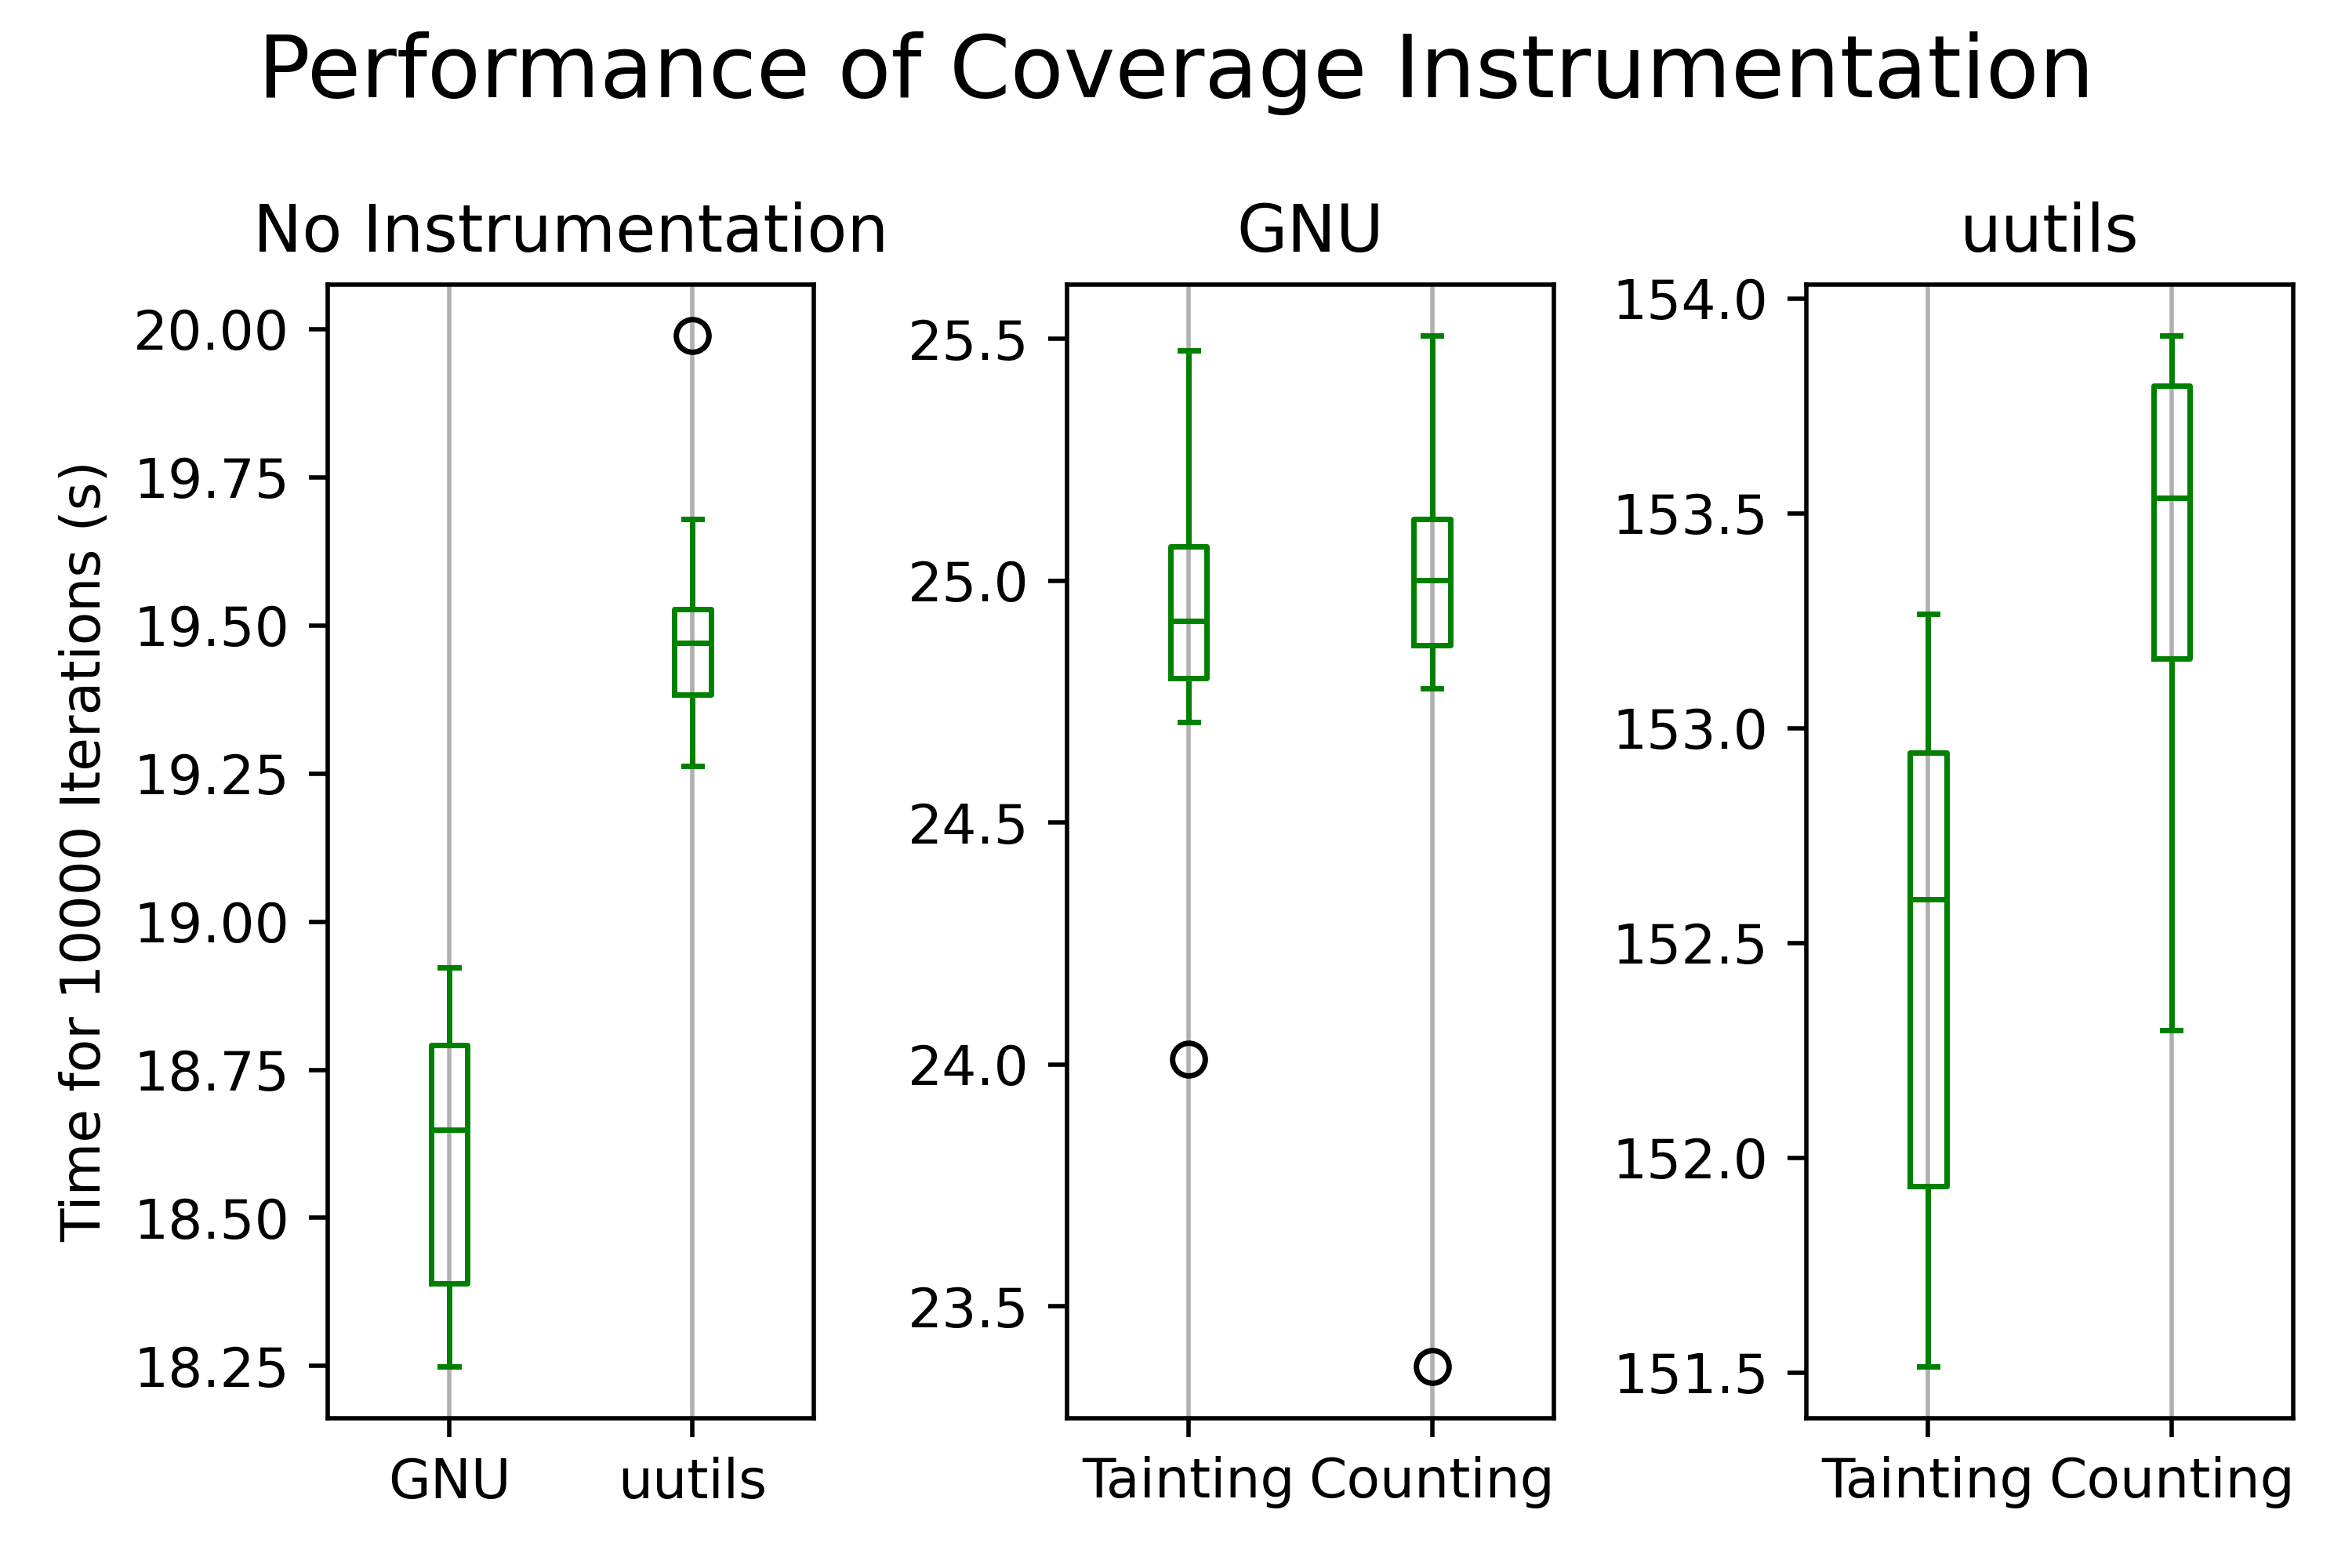
\includegraphics[width=\columnwidth]{assets/instrumentation.png}
            \captionof{figure}{Performance Implications of Coverage Instrumentation}
            \label{fig:coverage-instrumentation}
        }

    The reason why clang produces a greater number of edges in Rust code compared to C code, at least for the discussed versions of \code{base64}, could not be evaluated in this project, but may be worthy of further investigation.

    As pipes have a maximum size in Linux, the input cannot always be passed to the program under test directly. To circumvent this limitation, the fuzzer will write the input to a temporary file in an in-memory file system and pass this file to the program under test. Figure~\ref{fig:stdin-types} illustrates the impact of this approach on performance. While the performance impact is minimal for small input data, this is not necessarily the case for larger input data, as illustrated in Figure~\ref{fig:file-write}.


    Figure~\ref{fig:dynamic-file-stdin} illustrates the impact of varying input sizes on the performance of \code{base64} in total. This includes the additional runtime shown in Figure~\ref{fig:file-write}, which demonstrates that the impact of writing the data to a file is an order of magnitude smaller than that of \code{base64}, and thus acceptable.

        {
            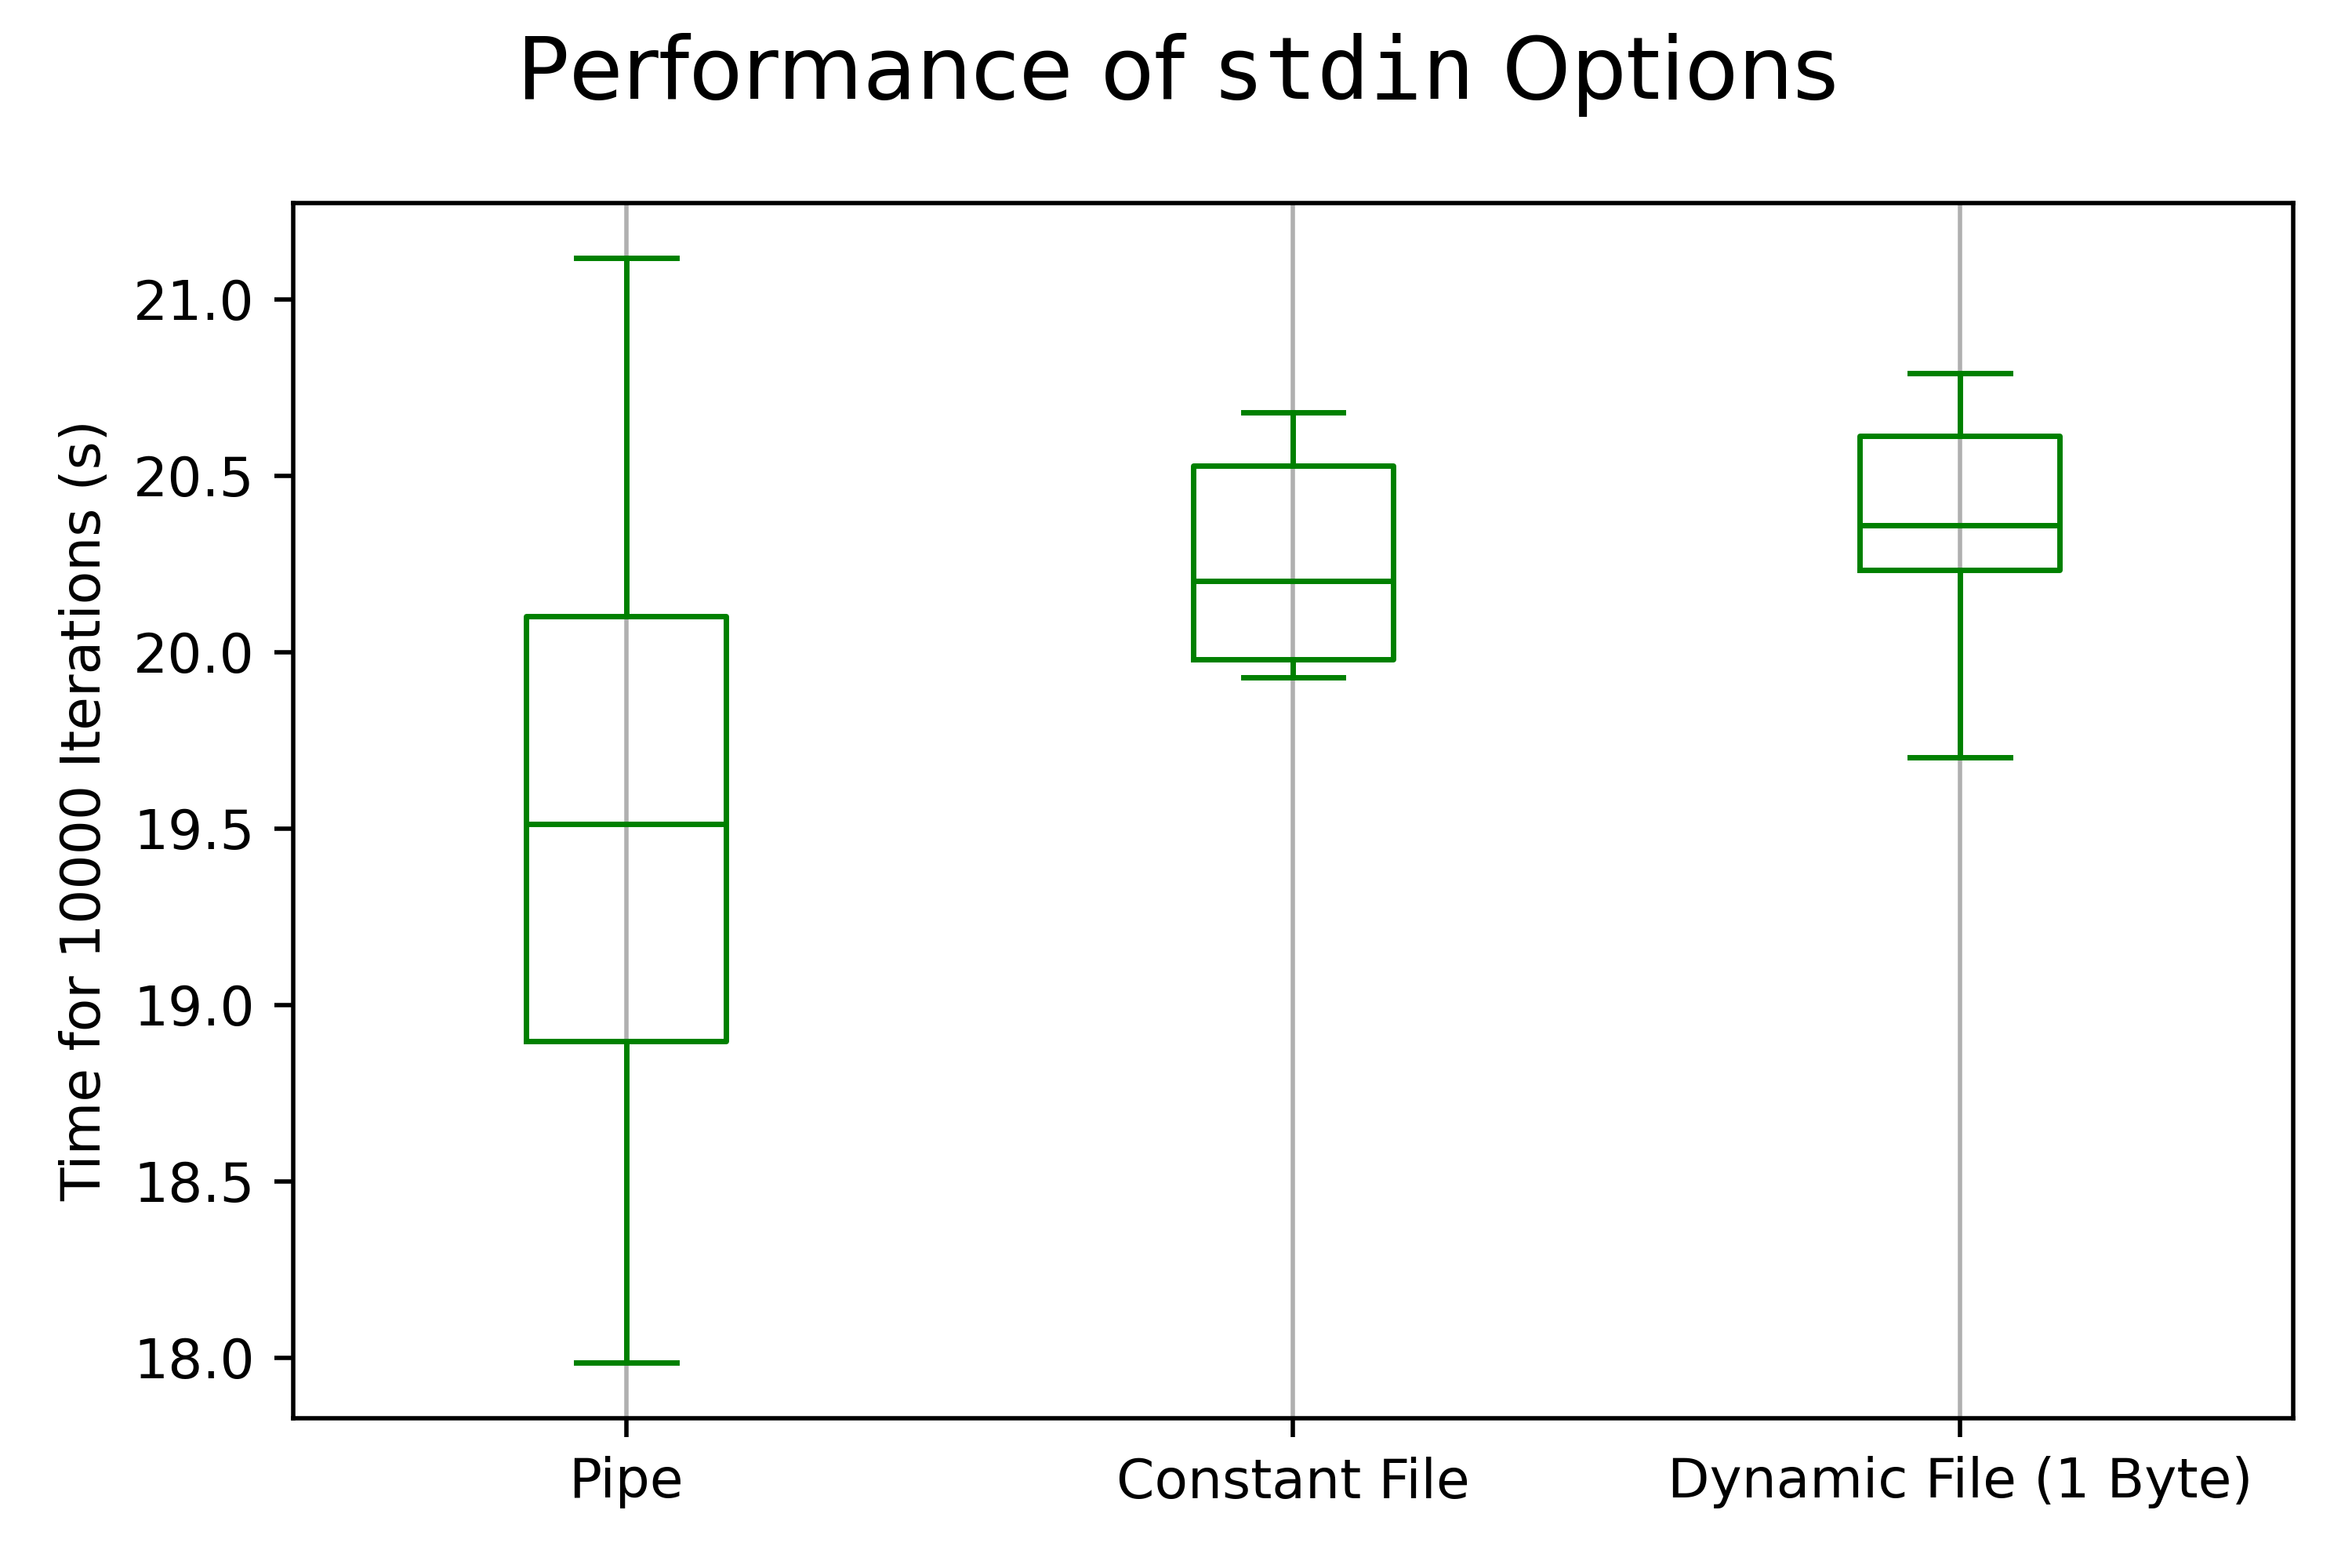
\includegraphics[width=\columnwidth]{assets/stdin_types.png}
            \captionof{figure}{Performance Differences When Passing Input Data to \code{base64} Directly, with a Default File, and with a File Created on each Execution}
            \label{fig:stdin-types}
        }


        {
            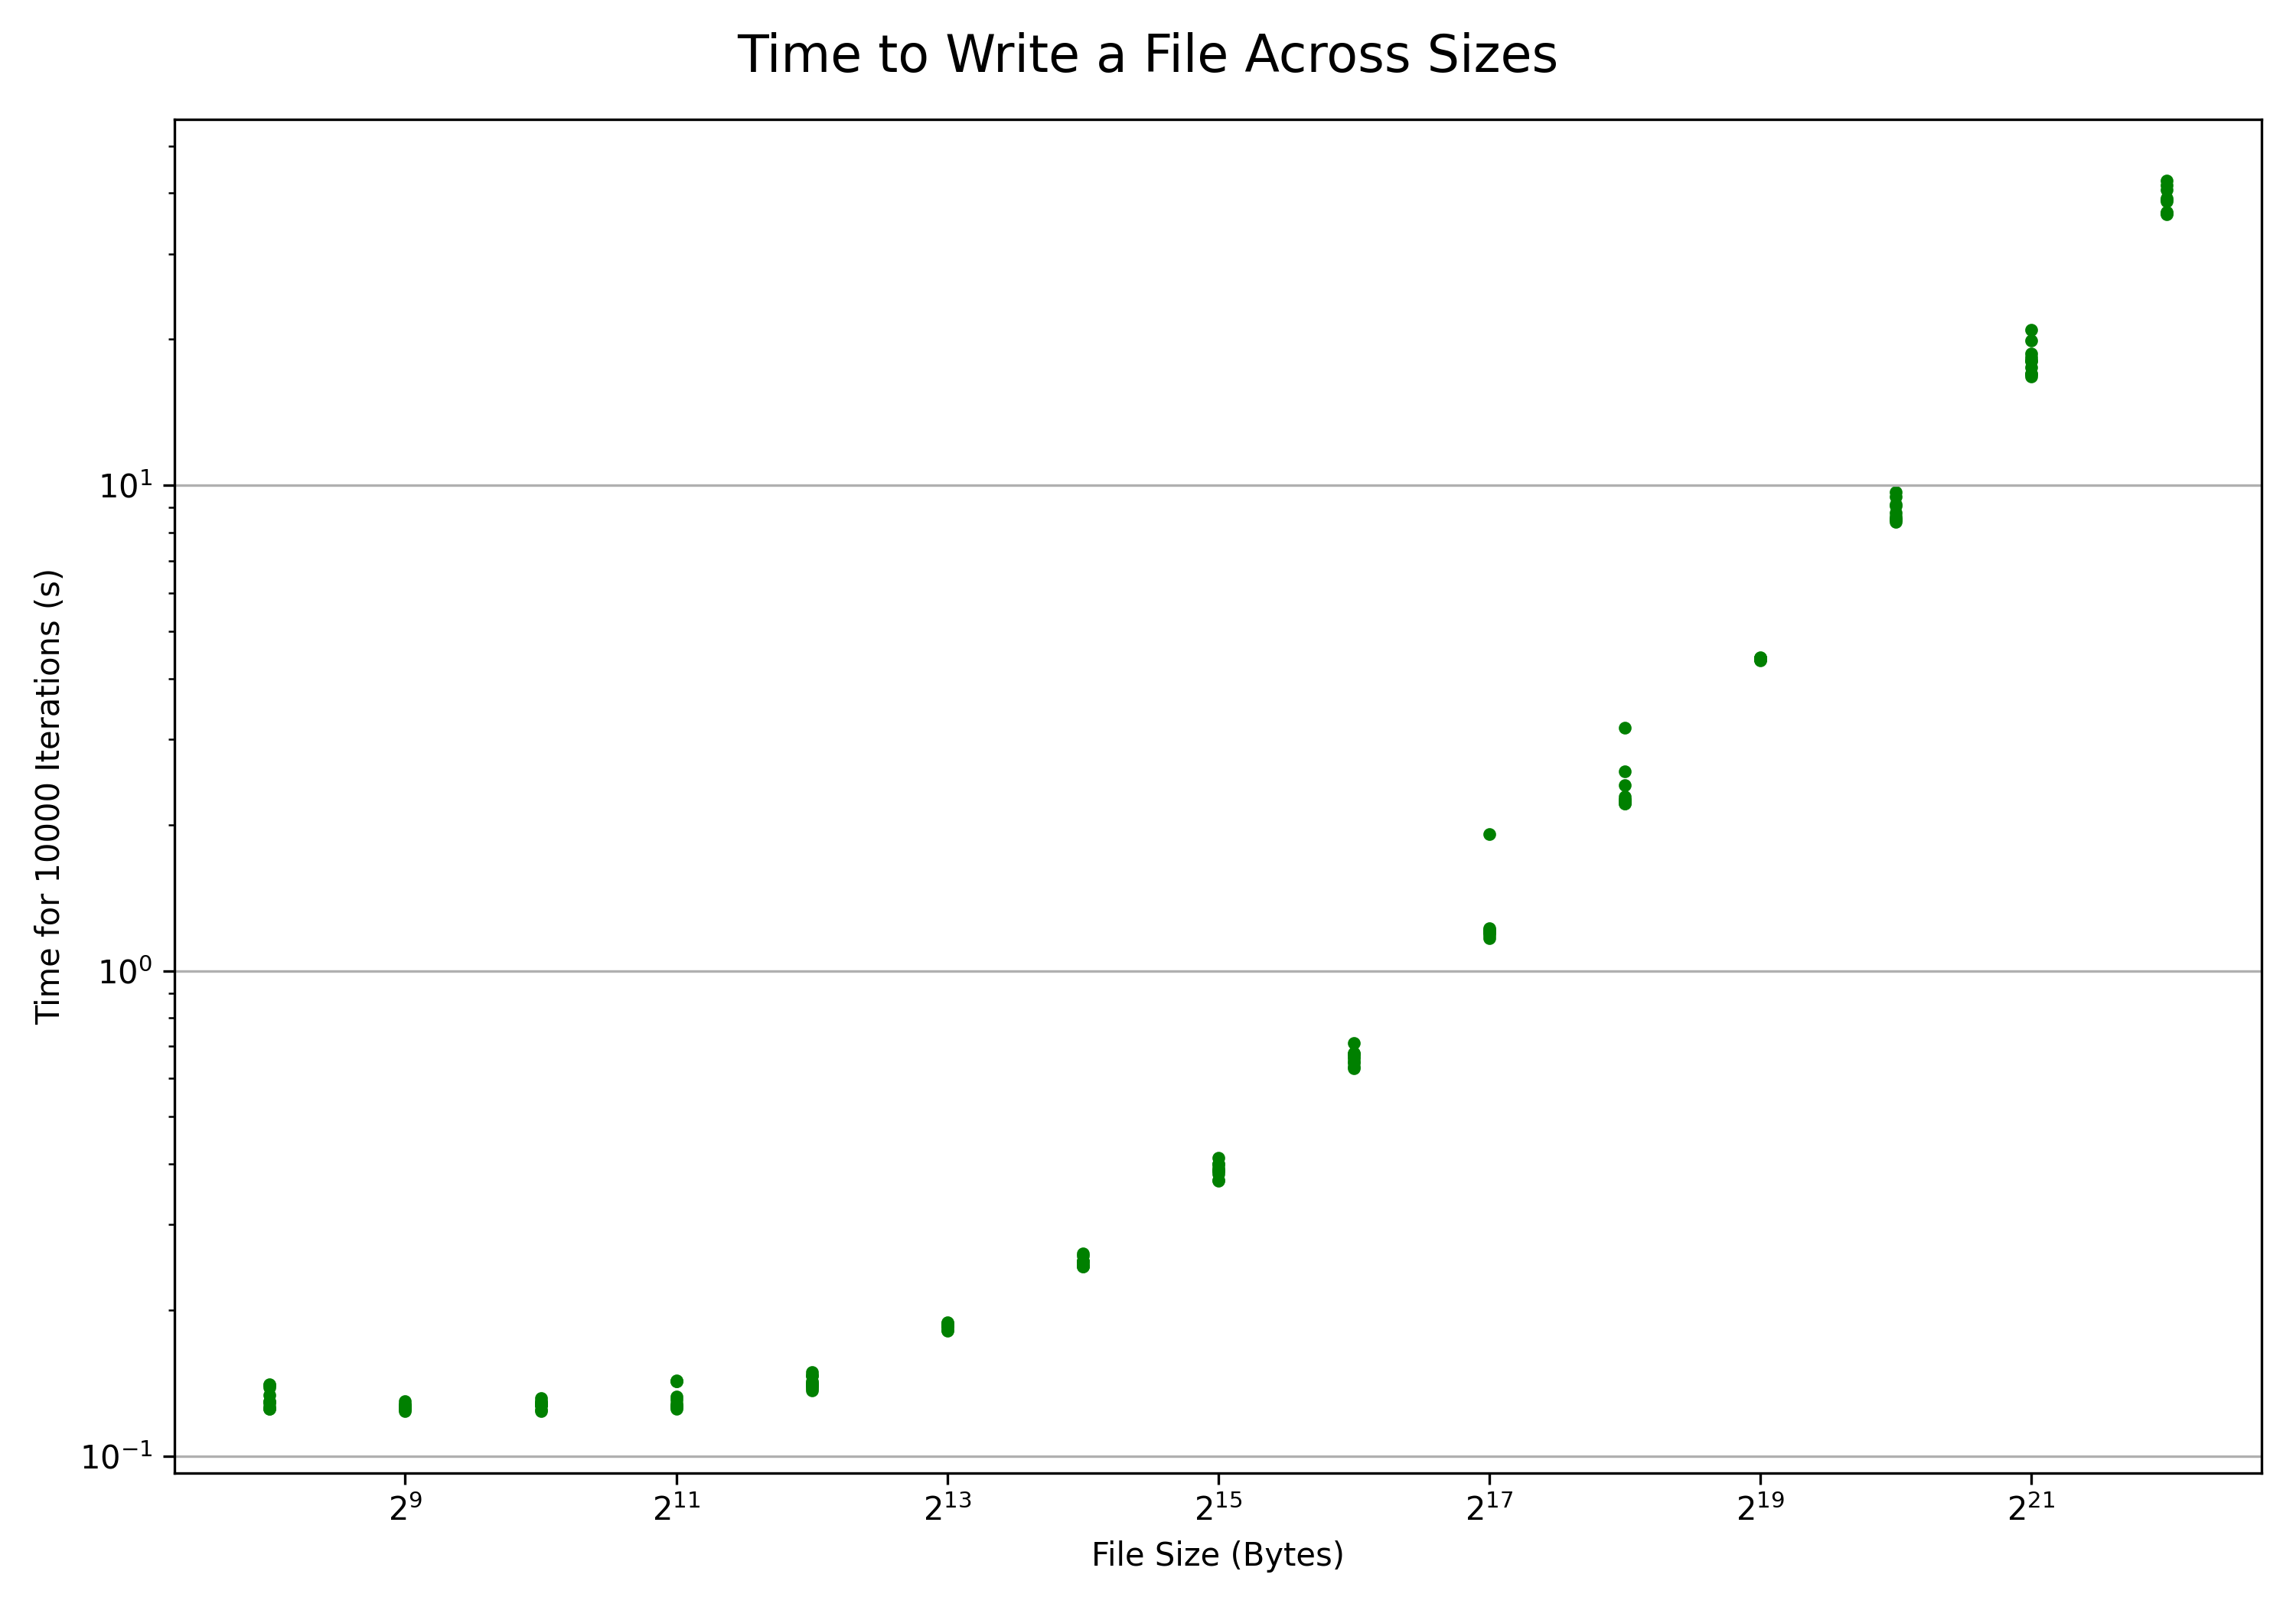
\includegraphics[width=\columnwidth]{assets/file_write.png}
            \captionof{figure}{Runtime Changes when Writing Differently Sized Files}
            \label{fig:file-write}
        }

        {
            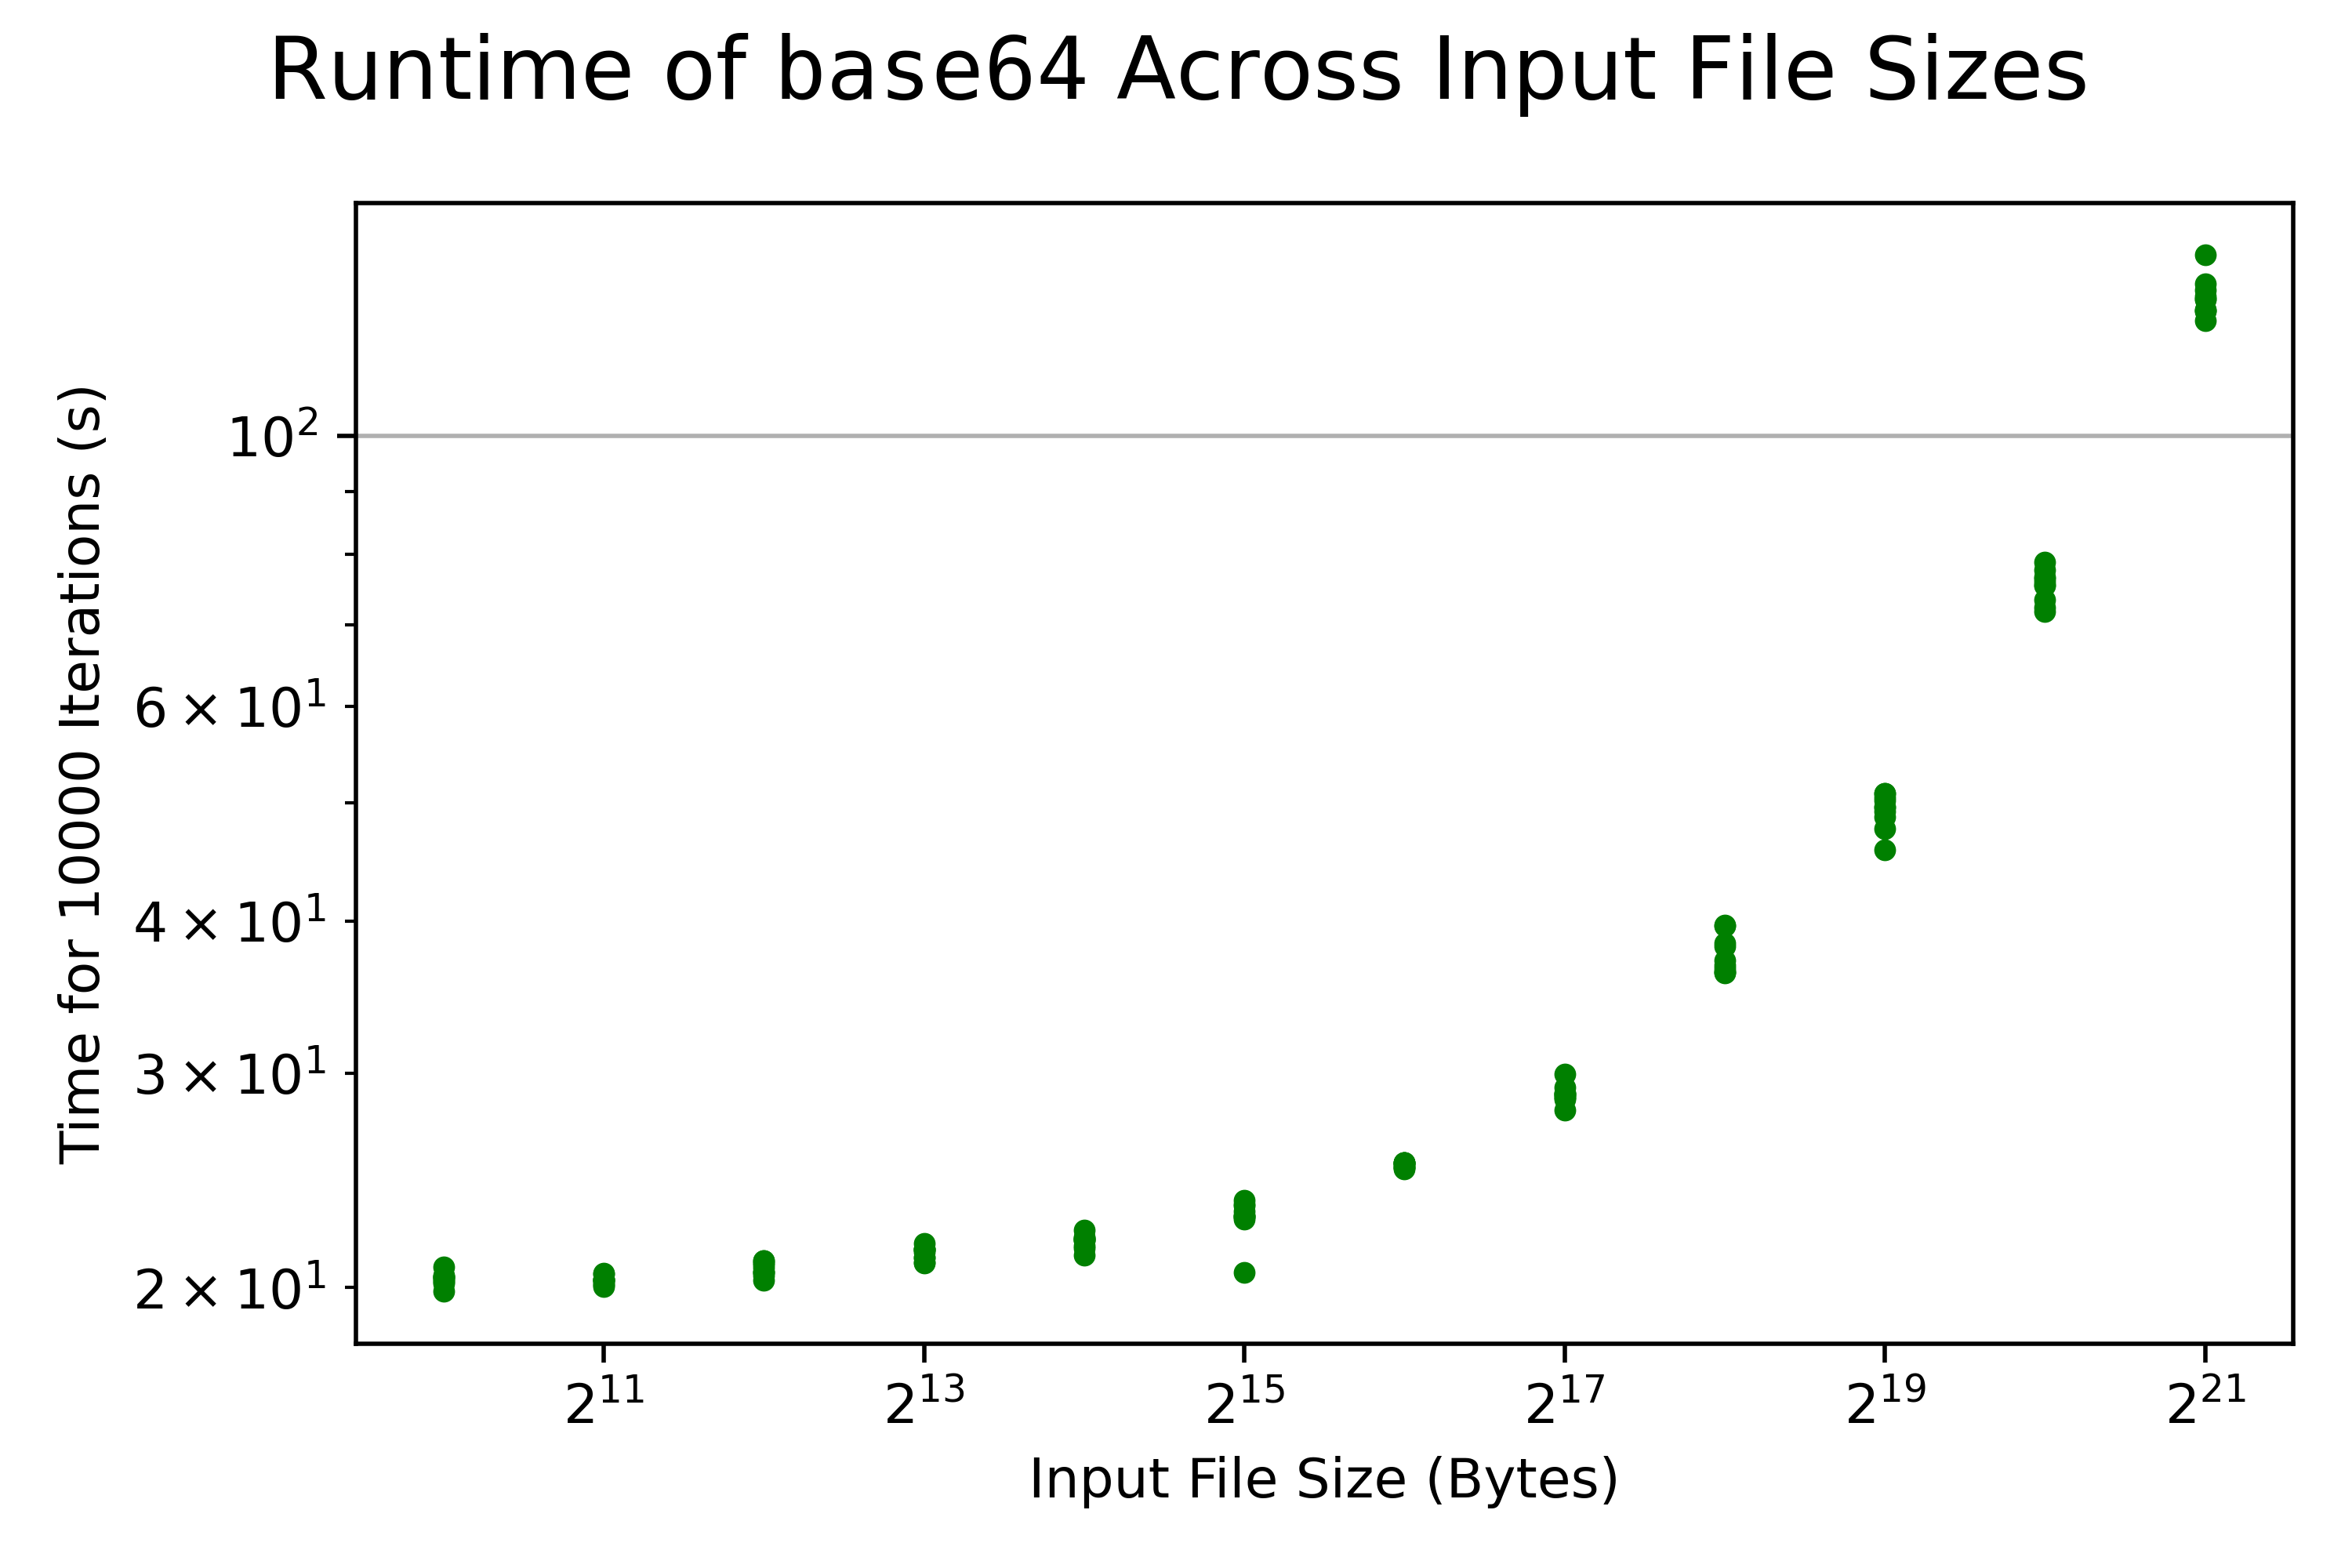
\includegraphics[width=\columnwidth]{assets/dynamic_file_stdin.png}
            \captionof{figure}{Runtime Changes when Executing \code{base64} on Inputs of Different Sizes}
            \label{fig:dynamic-file-stdin}
        }

    The Performance of shared memory as provided by the \code{MmapShmem} module in LibAFL is demonstrated in Figure~\ref{fig:shmem} to be comparable to writing an input file, thus eliminating the potential for problematic overhead. Finally, Figure~\ref{fig:preloads} presents the performance implications of hooking into the functions necessary for this fuzzer. Compared to the baseline, the first option merely hooks into \code{libc_start_main} and calls the program's main function with unaltered parameters. The second option also hooks into \code{libc_start_main}, but includes a hook for \code{rtld_fini} in its call to the main function. The hook in this example only calls the original \code{rtld_fini}, whereas the fuzzer uses this hook to copy coverage information to the shared memory.

    The overall performance of the fuzzers can be explained almost entirely by a combination of the aforementioned experiments, with the remaining runtime being introduced by minor additional logic such as output capturing.


        {
            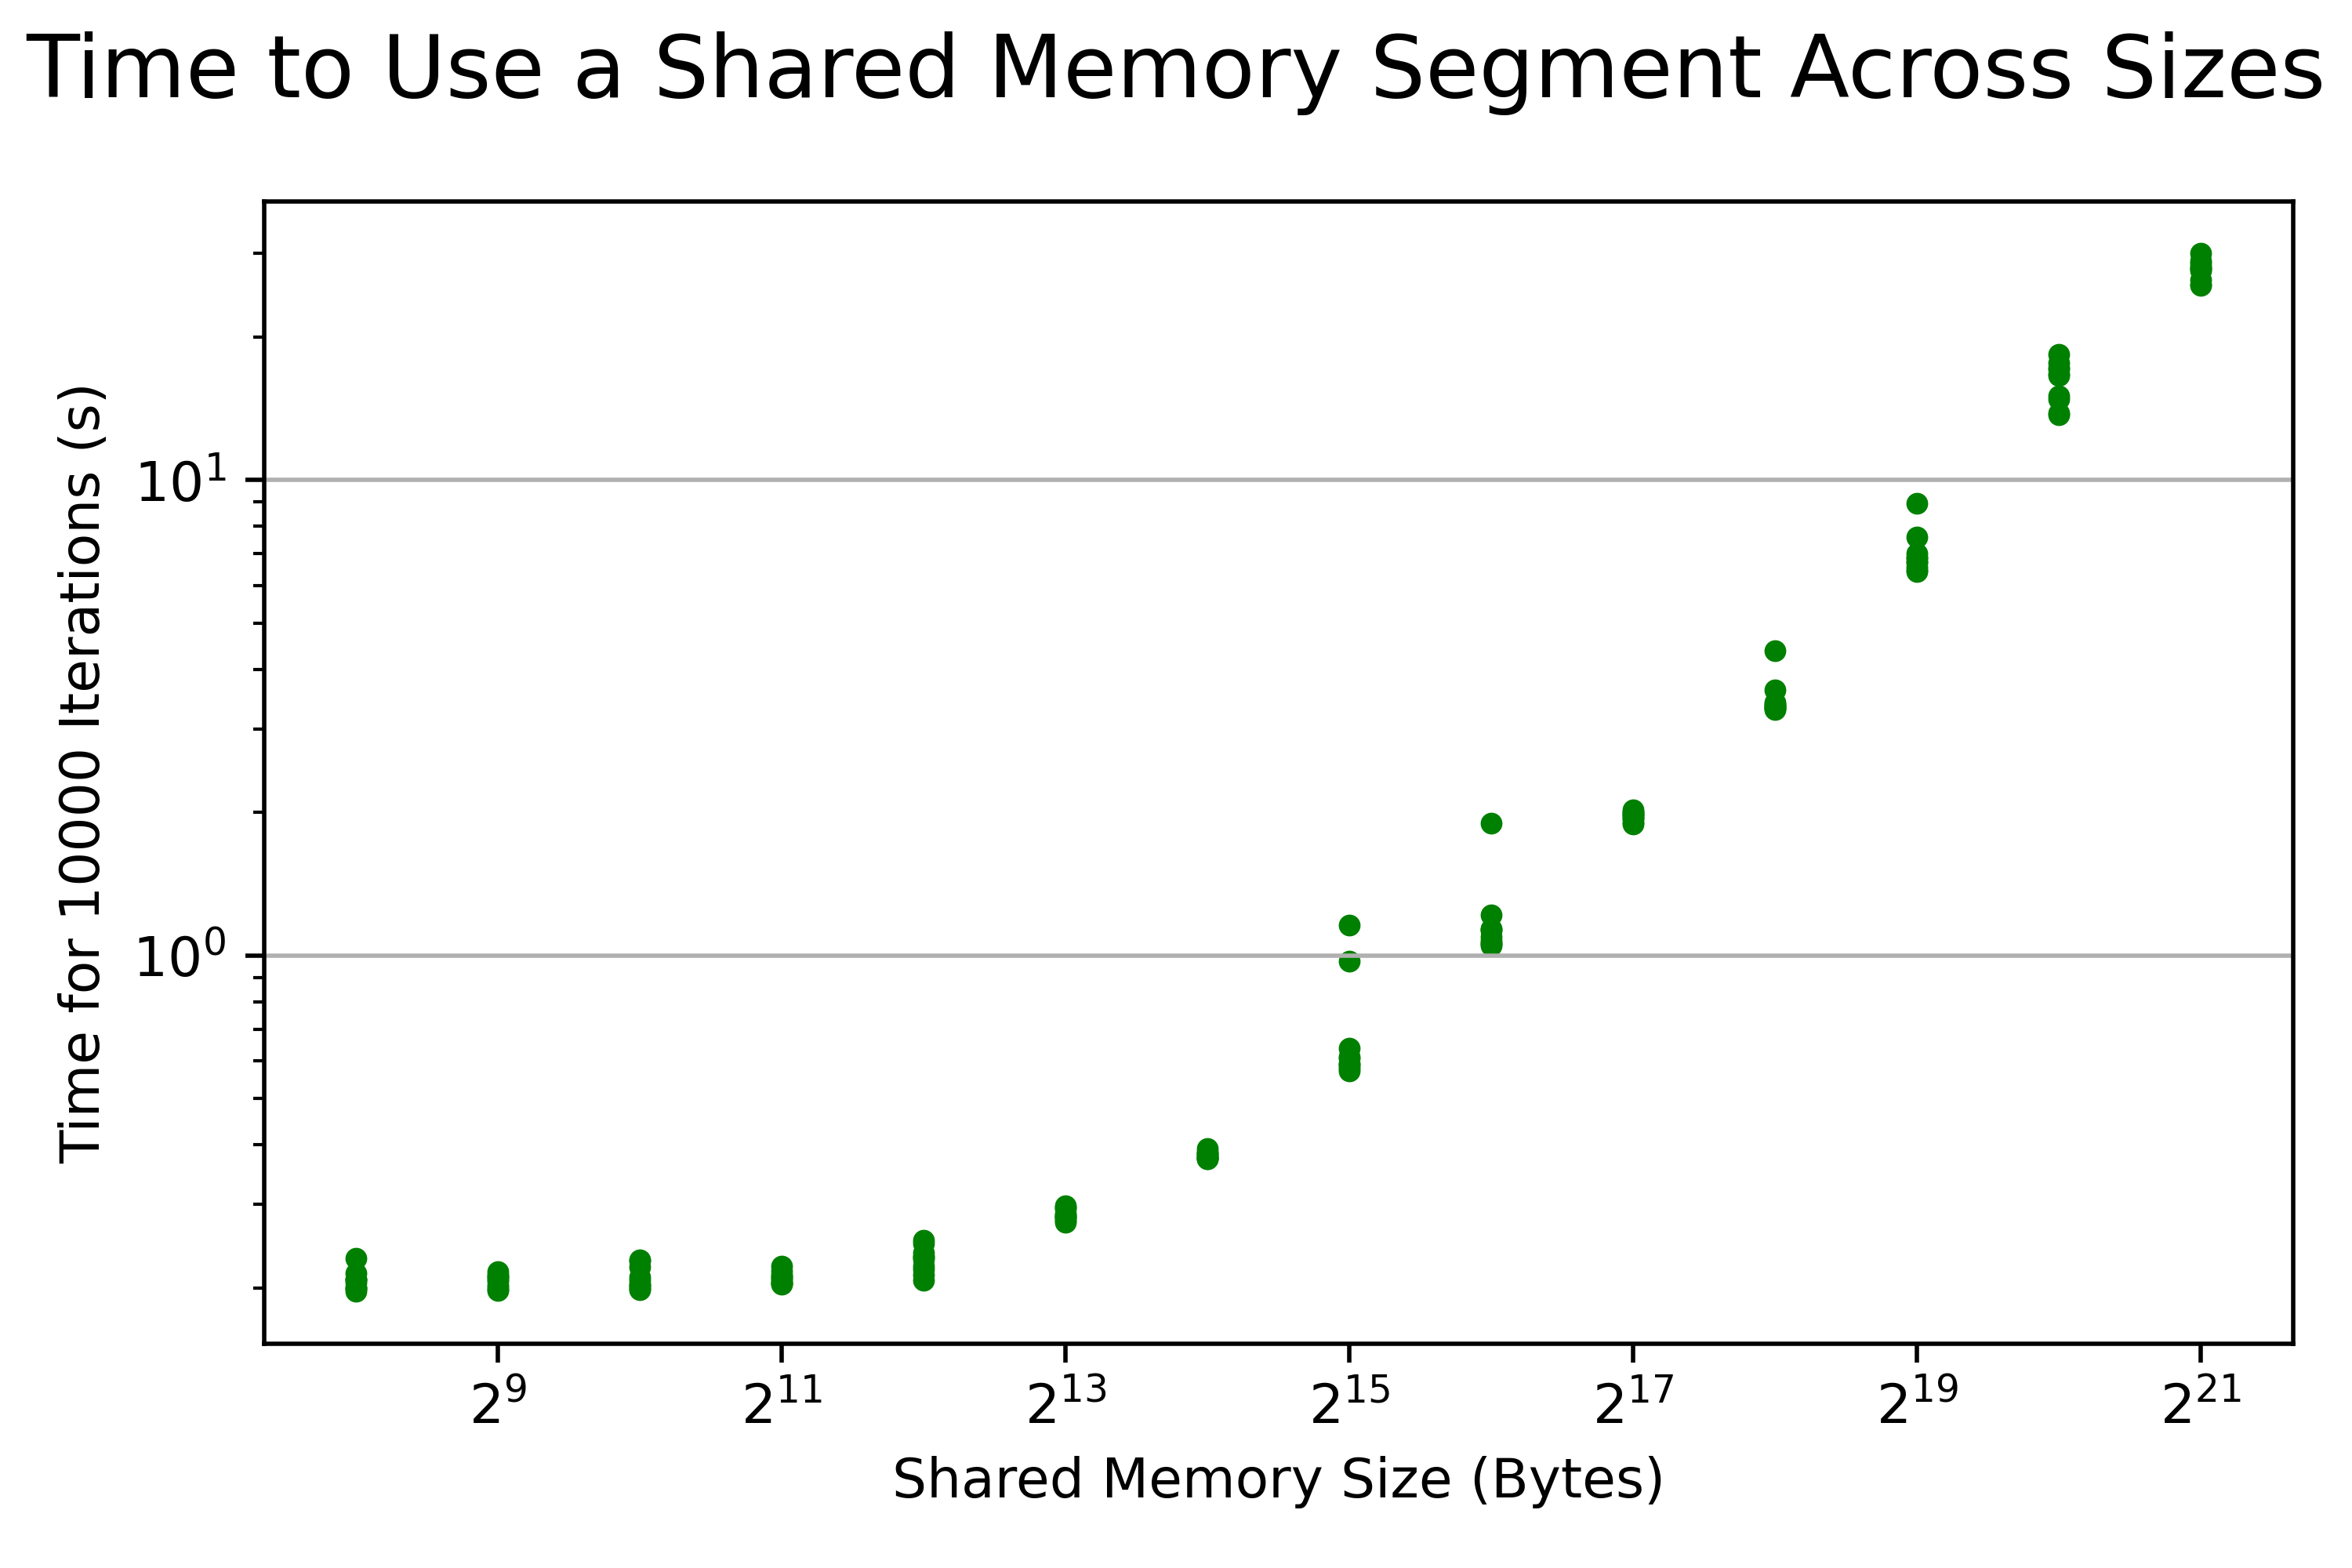
\includegraphics[width=\columnwidth]{assets/shmem.png}
            \captionof{figure}{Time to Allocate, Persist, Fill, and Check Shared Memory as Provided by \code{MmapShmem}}
            \label{fig:shmem}
            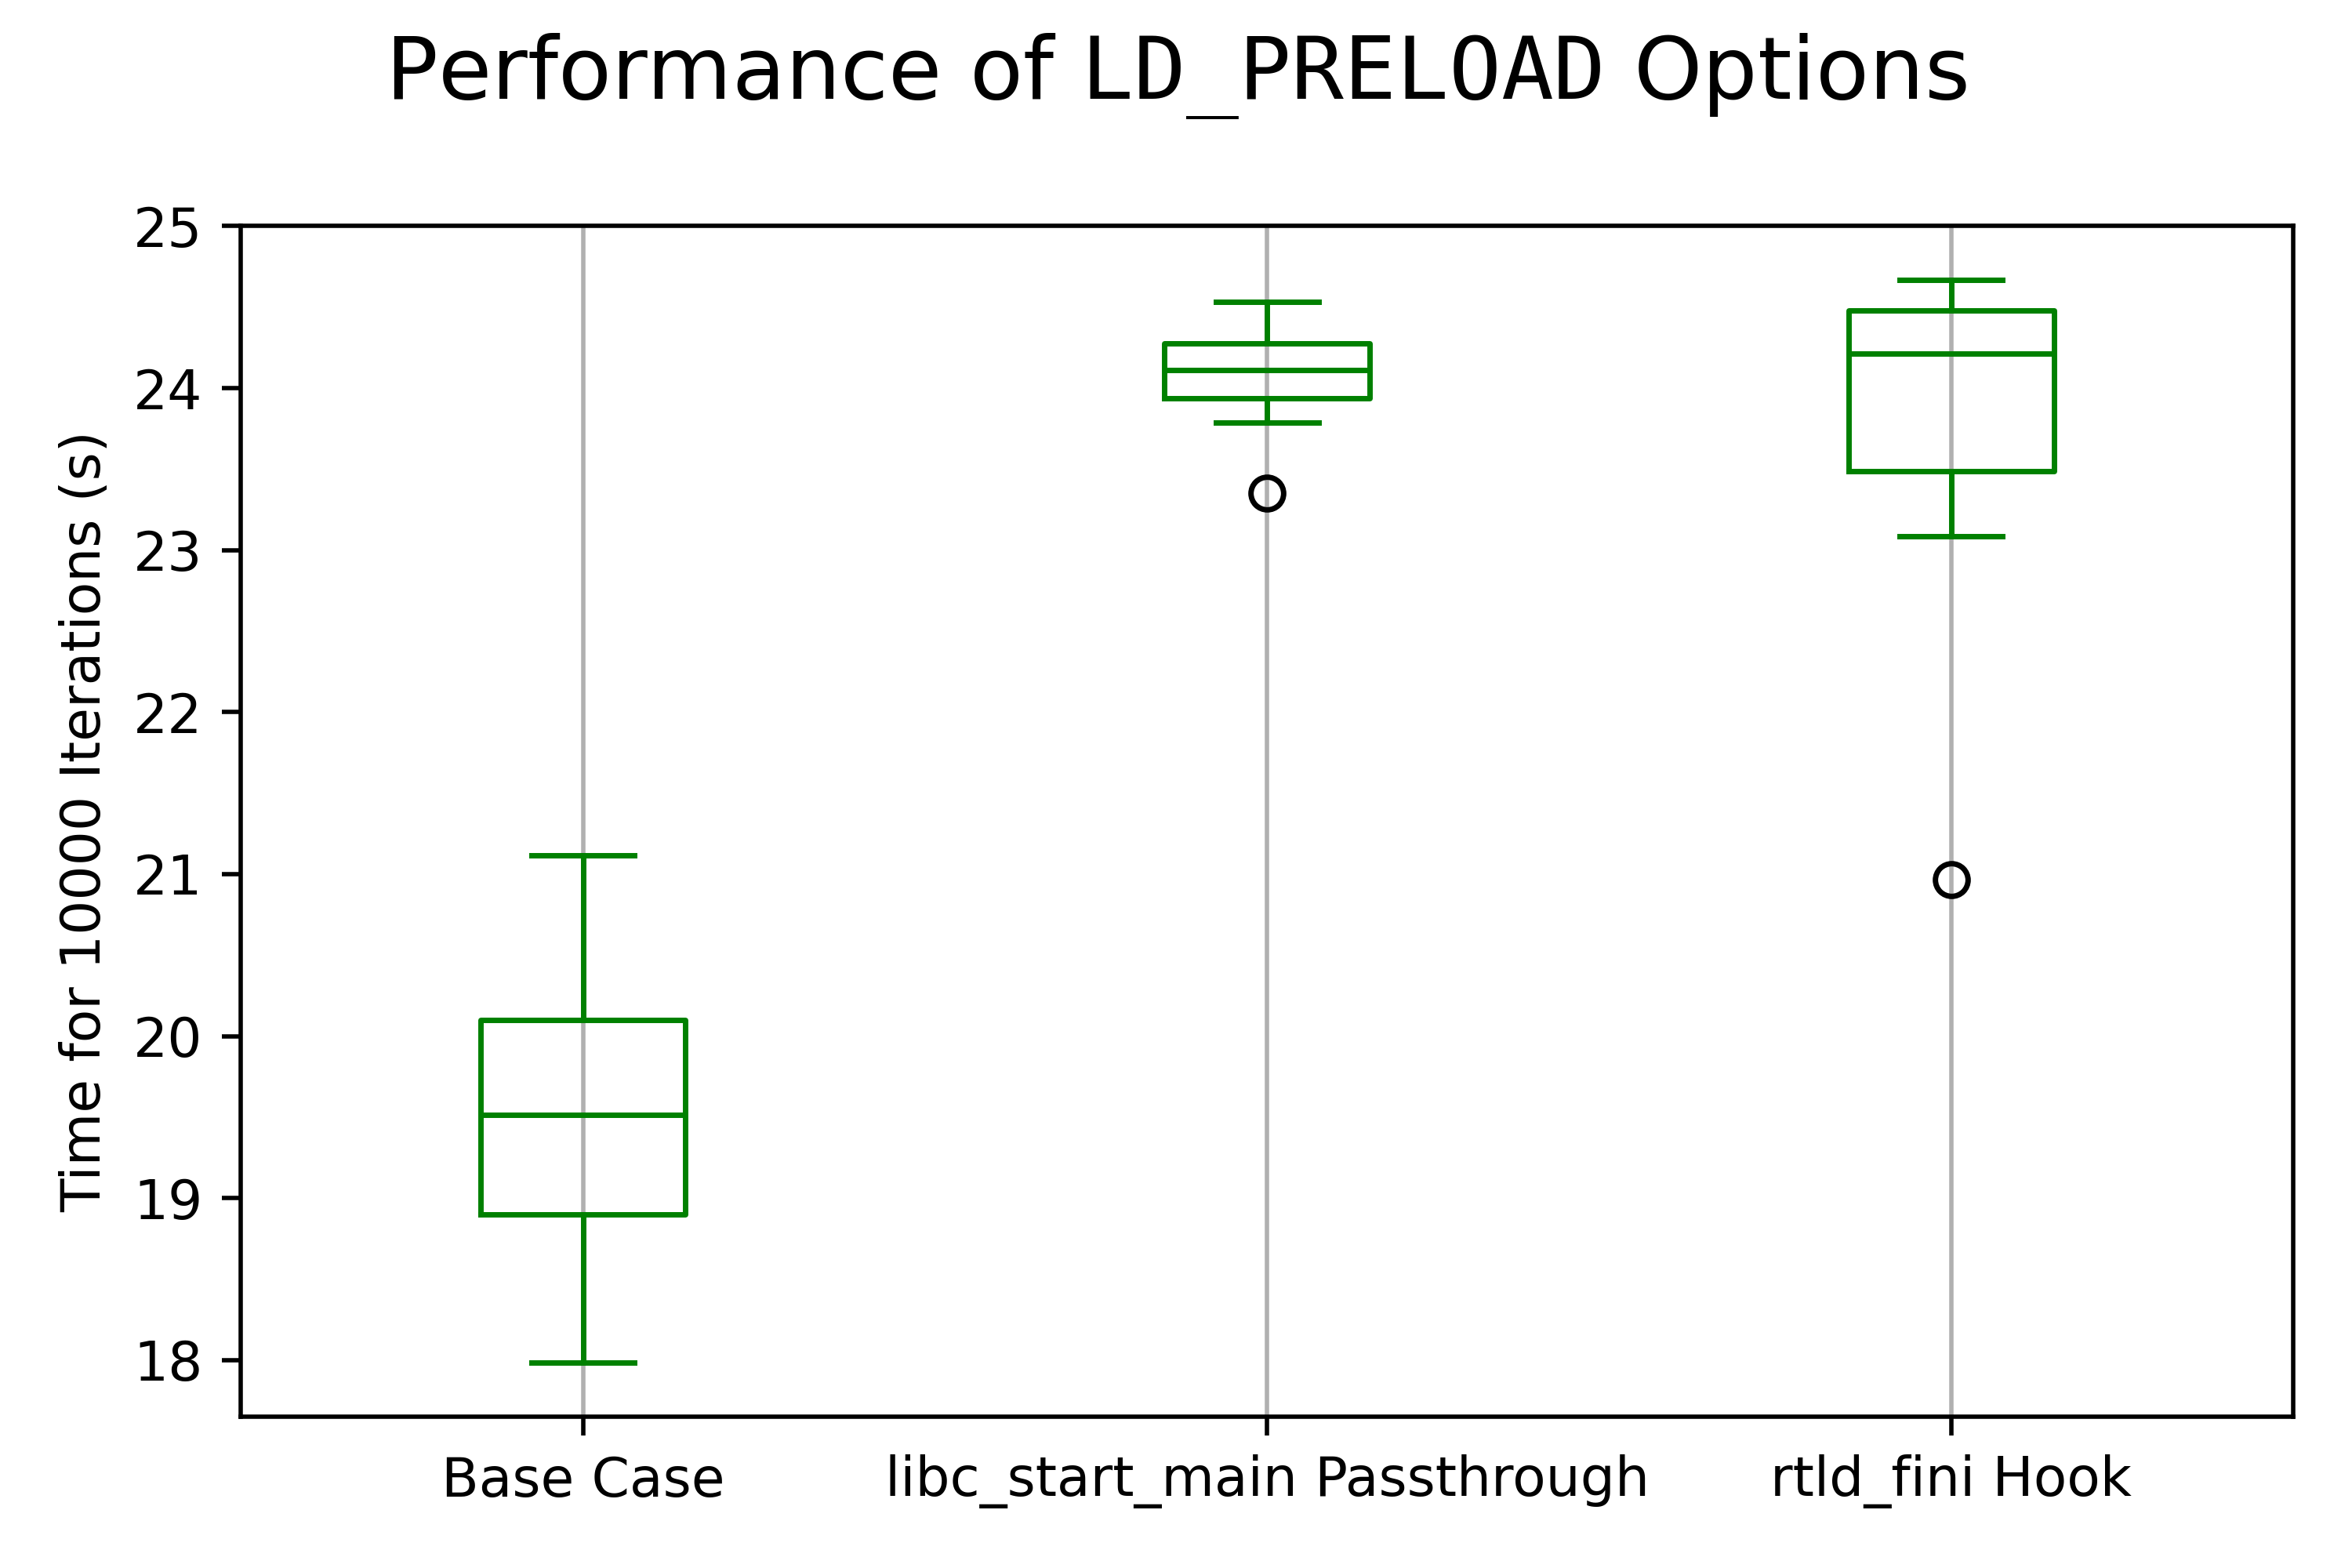
\includegraphics[width=\columnwidth]{assets/preloads.png}
            \captionof{figure}{Performance Impact of \code{LD_PRELOAD}}
            \label{fig:preloads}
        }

    \subsubsection{Coverage}

    According to the fuzzer, only 9.854\% of edge coverage is reached in its differential mode. To gather additional information about this number, the GNU coreutils were additionally compiled with instrumentation for coverage analysis with \code{gcov}. The fuzzer was then instructed to execute \code{Input}s, that reached new edges on this version of the program under test. This is accomplished by introducing a new \code{Feedback}, which can be attached to the \code{MaxMapFeedback} using Boolean logic operators in a way it is only evaluated when the \code{MaxMapFeedback} considers the \code{Input} interesting. This new \code{Feedback} evaluates all \code{Input}s as interesting and simply runs the \code{gcov} instrumented binary with the current \code{Input}. This results in only 1690 executions on an evaluation run with millions of executions on the binaries under test, thus introducing negligible performance overhead.

    \columnbreak

    An analysis of the results reported by \code{gcov} shows that 61.49\% of 161 lines were executed. After manually invoking \code{base64} with its \code{--help} and \code{--version} flags, gcov reported 83.23\% coverage. Manual inspection of the coverage file showed that the missing lines consist of \code{stdio} error handling code (e.g. write operations to \code{stdout}, which should never fail, since pipes are not intentionally broken by the fuzzer).

    \subsubsection{Performance on Individual Implementations}
    \label{IndividualFuzzers}

    The fuzzer is constructed in a manner that allows it to be run on a single implementation. As described in Sections~\ref{IntroductionDifferentialFuzzing} and~\ref{DifferentialFuzzing}, this reduces the kind of software error that can be found to those that result in the program under test crashing. Given that the runtime of \code{base64} it is not possible to discover infinite loops based on program runtime, since the execution timeout would need to be impractically long to ensure the absence of false positives.

    As anticipated from the experiments shown in Figure~\ref{fig:coverage-instrumentation}, the fuzzer performed significantly better on GNU's version of coreutils, achieving a 5.1 times higher execution rate. The discrepancy in the execution speed between the fuzzer and manual tests can be attributed to the additional computational processes inherent to the fuzzer, such as coverage analysis. The enhanced child process management in  \code{CommandExecutor}, as employed by the fuzzer, further optimises the execution speed, reaching a point where the fuzzer achieved almost twice the execution count compared to manual tests within the same time frame.

    The fuzzer did not identify any input that could cause crashing errors in either the GNU or uutils versions of coreutils.

    \subsection{Discovered Errors}
    \label{Errors}
    In an evaluation run spanning 24 hours and encompassing nearly 100 million executions, the fuzzer was unable to identify any errors in \code{base64} from either version of coreutils, neither in its individual or differential mode. However, GNU's version of \code{base64} comprises 161 lines of code according to \code{gcov} including its user interface. Given its extensive usage and the number of individual who have tested the code, it is highly improbable that there are any errors in the code base to begin with.

    To assess the efficacy of this fuzzer in identifying logic errors, an artificial bug was introduced into the source code of GNU's version of \code{base64} (see Listing~\ref{listing:artificial-bug}). This bug does not result in the program crashing or entering a state that would be flagged as a bug by conventional fuzzers. The fuzzer developed in this project identified this bug within minutes on multiple runs. This demonstrates that even bugs that have complex requirements on the input that trigger them can be found with this approach.

        {
            \begin{lstlisting}[language=C]
void base64_encode(const char *restrict in, idx_t inlen, char *restrict out, idx_t outlen)
{
if (inlen == 3)
    if (in[0] == 'a')
        if (in[1] == 'b')
            if (in[2] == 'c')
                printf("Hello, World!");

[remaining function code]
}
\end{lstlisting}
            \captionof{listing}{Inserted Artificial Bug}
            \label{listing:artificial-bug}
        }


    \section{State of the Art}
    \label{StateOfTheArt}

    This is not the first project to employ differential fuzzing techniques nor the first to fuzz coreutils. This section introduces previous works and discusses their limitations compared to this project.

    \subsection{uutils' Fuzzing Sub-Project}

    The only other project that performs differential fuzzing on coreutils is within the uutils coreutils repository. It contains code to fuzz 16 programs, 11 of which perform differential fuzzing against the system installation of the appropriate program from GNU coreutils.

    libFuzzer is used as a fuzzing backend, which integrates with cargo and provides coverage instrumentation. However, the interface of libFuzzer is currently limited to the \code{fuzz_target} macro, which only supports input types in the shape of simple byte arrays. In the project in its current state, this input is not used in combination with differential fuzzing. For those programs, the input is manually randomly generated, thus negating any advantage that coverage-guided fuzzing introduces.

    Only for the non-differential fuzzers, the input provided by libFuzzer is used. Of the five fuzzing binaries in this category, four do not test entire programs but instead import parsing routines. The sole exception is \code{date}, where actual coverage-guided fuzzing on a full program from coreutils is performed. The command line arguments are generated from the byte array input by splitting at \code{NULL} bytes. This is not a generally viable strategy, as is argued in Section~\ref{Environment}.

    Overall, compared to uutils' fuzzing sub-project, this work performs both coverage-guided and differential fuzzing simultaneously, while utilizing the flexibility gained by building on top of LibAFL to increase performance and ensure environment protection and thus reliable testing.

    \subsection{Fuzzing coreutils}

    The seminal work that introduced fuzz testing to the scientific community tested a suite of utilities on different UNIX systems, including some that would later be found in coreutils. Their system was very simple: generate random data (either completely random, random data without \code{NULL} bytes, or random printable characters) and check if the utility crashes. By undertaking this approach, the researchers identified errors in between a quarter and a third of utilities, depending on the UNIX system.\cite{UNIX}

    The authors later repeated their experiments, most recently in \citedate{UNIXRevisited}. However, they still followed a black-box fuzzing approach with no execution guidance or other techniques developed in the past 30 years. Additionally, the authors tested the uutils implementation and found similar levels of error prevalence.\cite{UNIXRevisited}

    \subsubsection{Symbolic Execution Frameworks}

    KLEE is a symbolic execution-based whitebox fuzzer that relies on SMT solvers to calculate inputs that will traverse new paths in a program. This approach has been shown to be highly effective at achieving high coverage in both the GNU and BusyBox versions of coreutils.\cite{KLEE} Additionally, KLEE forms the foundation for a list of fuzzers that build upon its capabilities to introduce novel concepts. Some notable examples include:

    \begin{itemize}
        \item CRETE introduced the concept of concolic execution, whereby the program under test is run with concrete values and the instructions executed are traced to subsequently calculate new inputs based on this instead of keeping the entire state-space in memory.\cite{CRETE}
        \item FUSE only selectively performs symbolic execution based on function complexity analysis.\cite{FUSE}
        \item Learch introduced a state selection algorithm that learns which state contributes most towards maximizing coverage.\cite{Learch}
        \item Cloud9 proposed a custom state-merging algorithm to help mitigate the state-explosion problem inherent in symbolic execution.\cite{Cloud9}
    \end{itemize}

    \subsubsection{Other approaches}

    Outside of symbolic execution-based fuzzing, coreutils have received little attention in academia. The following works were identified:

    \begin{itemize}
        \item CLIFuzzer\cite{CLIFuzzer} automatically extracts information about the command line interface from the program in question and then generates inputs based on this grammar. However, it does not take coverage information or any other guidance heuristic into account.
        \item AFL included an argv fuzzing mode, however, according to the author, \textquote{it's just not horribly useful in practice}\cite{AFLPlusPlusargv}. \citeauthor{AFLCoreutils} attempted to evaluate its effectiveness, but showed the drawbacks outlined in Section~\ref{Environment}.\cite{AFLCoreutils}
    \end{itemize}

    \subsubsection{Other Related Works}

    Finally, certain loosely fuzzing-related projects make use of coreutils in some part of their evaluation:

    \begin{itemize}
        \item SEDiff performs differential fuzzing on coreutils, but is not looking at software errors in the programs itself but instead evaluates function summaries used in symbolic execution based fuzzing.\cite{SEDiff}
        \item \citeauthor{DarpaExtended} evaluates the top vulnerability discovery tool from the DARPA Cyber Grand Challenge on more complex programs that are closer to what is expected in real-world software. They use coreutils to evaluate prevalence of C library functions in real-world software.\cite{DarpaExtended}
        \item IMF-SIM is an attempt to de-obfuscate programs by comparing a vector calculated based on the behaviour of them. This vector is generated by a fuzzing-like process. The authors evaluate their approach on coreutils.\cite{IMF-SIM}
        \item Building seccomp filters for Linux sandboxing manually is a tedious and error-prone task. \citeauthor{Seccomp} employs a fuzzer-like program to automatically generate all possible syscalls from a program.\cite{Seccomp}
    \end{itemize}

    \subsection{Differential Fuzzing}

    Since differential fuzzing can only be performed on targets where two implementations are available that claim to include the exact same functionality, certain categories of such programs appear in literature.

    \subsubsection{Network Protocols}

    Given that the interface of network protocols must be well-defined for compatibility between different systems, and that the diverse ecosystem of network-attached systems produces multiple implementations of software stacks to handle such network protocols, this is an obvious target for differential fuzzing. Examples include testing Deep Packet Inspection (DPI) evasion for QUIC\cite{DPIFuzz}, errors in recursive DNS resolvers\cite{ResolFuzz}, or request smuggling through HTTP proxies\cite{T-Reqs}. Additionally \citeauthor{ParDiff} extract finite state machines from different implementations of 14 network protocols and perform differential fuzzing to find errors in them.\cite{ParDiff}

    \subsubsection{Cryptography Libraries}

    Cryptography libraries represent another potential target for differential fuzzing, given that the underlying logic is well-defined and multiple implementations exist (as evidenced by the 37 different implementations tested in\cite{TLS}). Examples include TLS handshake testing\cite{ExploitingDissent, TLS}, or TLS/SSL certificate validation\cite{NEZHA}.

    \subsubsection{Compilers and Interpreters}

    Despite the similarities between different JavaScript engines, there remain significant differences, due to unspecified behavior. However, \citeauthor{JIT-Picking} perform differential fuzzing on JavaScript engines by comparing their interpreter to their just-in-time (JIT) compiler.\cite{JIT-Picking}

    In\cite{JVM} and\cite{JVM2}, the authors test different Java Virtual Machine (JVM) implementations against each other to find 92 bugs in total. \citeauthor{WASM} tests different WebAssembly interpreters\cite{WASM}, while \citeauthor{UndefinedBehavior} attempt to find undefined behavior based bugs in compilers\cite{UndefinedBehavior}. Another project trained a machine learning system to generate realistic programs as inputs for different compilers.\cite{CompilerDL}

    Similarly, EVMFuzz compares different implementations of the Ethereum Virtual Machine.\cite{EVMFuzz} Fluffy attempts to create multi-transactional test cases for the Ethereum network that exploit consensus bugs in different implementations to trigger hard forks of the network.\cite{Fluffy} Other networks tested include the Neo blockchain in NeoDiff.\cite{NeoDiff}

    \subsubsection{Regression Testing}

    Differential fuzzing can also be employed in the context of regression testing. This approach has the significant advantage of not necessitating two different implementations of the same logic, as two versions of a program are tested against each other. This methodology is only viable if the difference between the tested versions is limited to performance enhancements or other refactoring changes, as any alterations to functionality or the introduction or fixes of bugs would be caught by the fuzzer. Examples include work done by \citeauthor{HyDiff}\cite{HyDiff}.

    \subsubsection{Deep Learning}

    Deep learning systems remain still largely only superficially understood. Ensuring reliable operation is becoming ever more important as such systems are increasingly used in high-stakes environments such as self-driving cars. While the same approach of comparing multiple similar tools can be applied to deep learning systems as well, in works such as by \citeauthor{DLFuzz}\cite{DLFuzz}, the term differential fuzzing refers to the technique of adding minor noise to an input and checking if a classifier model returns the same output for the original and altered input. Similar to what is done in this project, coverage-guided fuzzing can be applied to deep learning models by counting activated neurons instead of executed edges.

    \subsubsection{Side-Channel Attacks}

    Finally, a different form of differential fuzzing can be employed to discover side-channel attacks. By comparing the resource consumption (e.g. time, memory, or energy) of the same program using two different inputs and mutating these inputs to maximise the difference, information about the program state can be retrieved, as demonstrated in\cite{DifFuzz}.

    \section{Discussion}

    This work presents a new fuzzer built on LibAFL, designed to perform differential fuzzing between different implementations of coreutils. Even though, because of current limitations in LibAFL, only a single program could be tested, it can be shown that this approach is promising in finding logic errors in programs such as \code{base64}. This section discusses the findings in this work, its contributions and limitations, and attempts to answer the research questions posed at the beginning.

    \subsection{Research Questions}
    \label{ResearchQuestionsDiscussion}
    Section~\ref{ResearchQuestions} introduced a series of questions to be answered in this work. Here is a summary of what was found.

    \begin{enumerate}
        \item In principle, all components of coreutils can be tested using a fuzzer. However, based on the interface information provided in Section~\ref{CoreutilsInterface} and the considerations on environment protection in Section~\ref{Environment}, a fuzzer designed to achieve complete coverage must introduce a computationally expensive layer to record environmental changes and prevent their persistence across executions of the program under test. Furthermore, a layer to emulate failed system interactions (such as broken pipes) must be implemented. The performance cost of these layers renders them impractical for use in testing without the availability of very large compute resources.
        \item This work introduces a novel approach to LibAFL for gathering coverage information from a binary called in a child process. Sections~\ref{CoverageGNU} and~\ref{Coverageuutils} describe how edge coverage is gathered by logic statically compiled into the binary under test and extracted by dynamically loaded libraries, transparent to the program under test.
        \item The fuzzer built in this project makes extensive use of LibAFL's features, including idiomatic usage of LibAFL's internal representation of coverage information (see Section~\ref{LibAFLCoverageInterface}), usage of advanced algorithms as provided by LibAFL (see Section~\ref{Optimizations}), and experiments on custom \code{Input} types (as described in Section~\ref{CustomInputType} and discussed in Section~\ref{CustomInputTypeLimitations}).
        \item A non-differential fuzzer is only able to find bugs that trigger states that are easily distinguishable from normal operation. Section~\ref{DifferentialFuzzing} explains why this in practice reduces the discoverable errors to those that either crash the program under test or produce timeouts. Section~\ref{IndividualFuzzers} demonstrates that even long evaluation runs on \code{base64} did not uncover any such bugs.
        \item Section~\ref{DifferentialFuzzingCode} outlines the existing functionality in LibAFL employed by the fuzzer in its differential mode, along with the custom extensions introduced during this project. Given LibAFL's modular design, running two \code{Executor}s in parallel, including all their respective \code{Observer}s, and introducing \code{Feedback}s comparing their output is not only feasible but also a relatively straightforward engineering task.
        \item Finally, the fuzzer in its differential mode is able to identify and locate artificially introduced non-trivial logic errors in the different implementations that are not discoverable by its non-differential mode. It explores all program parts, with the exception of those that have been excluded based on environmental protection reasons, as previously described.
    \end{enumerate}

    \subsection{Contributions}
    \label{Contributions}

    During the course of this project, a number of enhancements to LibAFL's upstream repository have been introduced:

    \begin{itemize}
        \item \code{CommandExecutor} was generalized to work on custom \code{Input}s, rather than simple byte array \code{Input}s only (\href{https://github.com/AFLplusplus/LibAFL/pull/2129}{PR~\#2129})
        \item Improvements to \code{StdOutObserver} and \code{StdErrObserver} (\href{https://github.com/AFLplusplus/LibAFL/pull/2236}{PR~\#2236})
        \item Introduction of \code{DiffExitKindFeedback}, which compares the \code{ExitKind} of two \code{Executor}s in differential fuzzing and reports discrepancies (\href{https://github.com/AFLplusplus/LibAFL/pull/2246}{PR~\#2246})
        \item A bugfix for \code{MmapShmemProvider} (\href{https://github.com/AFLplusplus/LibAFL/pull/2298}{PR~\#2298})
        \item Fixes to the handling of \code{StdOutObserver} and \code{StdErrObserver} and an example fuzzer to demonstrate their usage as part of a refactoring in collaboration with LibAFL's maintainers (\href{https://github.com/AFLplusplus/LibAFL/pull/2311}{PR~\#2311})
        \item
    \end{itemize}

    Based on feedback by the author of this work, the author in collaboration with LibAFL's maintainers began work on \code{tuple_list} and moving from \code{HasBytesArray} to \code{HasMutatorBytes}, in preparation of introducing \code{MappingMutator} to allow byte array mutation based on default \code{Mutator}s on arbitrary parts of a custom \code{Input}.

    Further improvements were discussed but could not yet be introduced because of time limitations, but may be in the coming months:

    \begin{itemize}
        \item \code{MappingMutator} as described above, including an example fuzzer showing handling of custom \code{Input}s
        \item A \code{CommandExecutor} implementation for custom \code{Input}s, where the mapping of \code{Input} parts to the different parts of the command is defined on the \code{Input} based on a trait
        \item A set of macros to automatically generate the mutators necessary for a custom \code{Input}
        \item An example fuzzer including possible further additions to LibAFL's source code to show how coverage information can be retrieved when using \code{CommandExecutor}, as done in this project
    \end{itemize}

    \subsection{Limitations and Future Work}

    Although the fuzzer introduced in the previous sections was already capable of producing results in the form of proof-of-concept work, it is subject to a number of significant limitations.

    \subsubsection{Untested Program Parts}
    Sections~\ref{CoreutilsInterface} and~\ref{ResearchQuestionsDiscussion} examine the limitations of the fuzzer in terms of its inability to test functionality that alters the environment. Furthermore, the handling of errors in the input and output of the programs (e.g. broken pipes) is not tested due to the absence of an intermediate layer that could introduce these errors artificially. Future projects may introduce these missing layers either individually or in combination, with the aim of testing the code sections not tested by this project.

    \subsubsection{Instrumentation Performance on uutils' coreutils}
    Section~\ref{PerformanceIndividualParts} discusses that while the performance between GNU's and uutils' version of coreutils is similar without instrumentation, adding coverage gathering logic increases the runtime of uutils' version by a factor of 8, compared to 1.3 for GNU's version. Future work may investigate the reason for this difference to improve this fuzzer's performance.

    \subsubsection{Limitations on Custom Input Type Mutations}
    \label{CustomInputTypeLimitations}
    Section~\ref{Results} explains why the evaluation of the fuzzer was only performed on \code{base64}. After the missing additions described in Section~\ref{Contributions}, specifically \code{MappingMutator} to mutate multiple byte array parts of a custom \code{Input} type, are introduced, a more complete evaluation will be possible.

    \subsection{Summary}

    This project introduces a new coverage-guided greybox fuzzer that performs differential fuzzing on coreutils. It builds on top and includes many advanced algorithms implemented in LibAFL while limiting the inputs it generates to those that ensure a constantly stable testing environment.

    A novel approach to transferring coverage information from a program executed as a separate process is employed, whereby the programs under test are extended with an interface to dynamically access coverage information without any changes to the source code. The system dynamically loads and links helper binaries during execution, providing coverage information in a manner that is idiomatically readable by LibAFL's coverage guidance modules.
    Due to incomplete functionality in LibAFL, the fuzzer produced in this project could only be evaluated on base64, where it achieved full coverage but did not discover any software errors. Further extensive tests will be required as a base for a full evaluation once the missing logic has been added to LibAFL.



\end{multicols}
\vspace{70px}
\begin{center}

    \begin{minipage}{0.7\textwidth}
        \centering
        In the interest of open science, this project is released under an open-source license. During development, over 500 lines of code have been introduced to the upstream project, with further major changes already in discussion. The source code of the project is publicly available at\\\vspace{8px}\href{https://github.com/riesentoaster/coreutils-differential-fuzzing}{https://github.com/riesentoaster/coreutils-differential-fuzzing}.
    \end{minipage}

\end{center}

\pagebreak

\begin{multicols}{2}
    \defbibheading{bibliography}[\bibname]{\section*{#1}}
    \addcontentsline{toc}{section}{\bibname}
    \printbibliography
\end{multicols}

\end{document}